\setcounter{saveenum}{\value{enumi}}
\begin{enumerate}
\setcounter{enumi}{\value{saveenum}}
\item Якщо $X$ та $Y$ --- незалежні , то
\end{enumerate}
{\centering
 $H(\normalsubformula{\textXY})=H(X)+H(Y)$.
\par}

З курсу теорії ймовірностей відомо визначення \textit{умовної ймовірності}:

{\centering
 $p\left(x |y \right)=\frac{p(x,y)}{p(y)}$,   $p(y)\neq 0$.
\par}

Нехай відомий результат  $y$ експерименту $Y$. Тоді можна визначити
умовну ентропію таким чином:

\begin{equation*}
{H\left(X |y \right)=-\underset{x\in X}{\sum
}{p\left(x |y \right)\log p\left(x |y \right)}}
\end{equation*}
Усереднивши  $H(X/y)$ за всіма  $y$, отримаємо \textit{умовну ентропію}
ансамблю  \textit{Х } відносно ансамблю $Y$ :

 $\begin{matrix}\underset{y\in Y}{\sum }?\hfill\null \end{matrix}{x\in
X}\hfill $

\liststyleWWviiiNumxxxix
\setcounter{saveenum}{\value{enumi}}
\begin{enumerate}
\setcounter{enumi}{\value{saveenum}}
\item \begin{equation*}
{H(X|Y)\ge 0}
\end{equation*}
\item \begin{equation*}
{H(\normalsubformula{\text{XY}})=H(X)+H(Y|X)=H(Y)+H(X|Y)}
\end{equation*}
\end{enumerate}
Інтуїтивно: сукупна невизначеність експериментів $X$ та $Y$
дорівнює невизначеності $X$ плюс невизначеність $Y$, що
залишилася після того, як результат експерименту $X$ став відомим.
$X$ та $Y$ входять у формулу симетрично.

\liststyleWWviiiNumxxxix
\setcounter{saveenum}{\value{enumi}}
\begin{enumerate}
\setcounter{enumi}{\value{saveenum}}
\item  $H(X)\ge H(X|Y)\ge H(X|\normalsubformula{\textYZ})$…
\end{enumerate}
Додаткові знання не можуть збільшити невизначеність.


\bigskip

\textit{Означення.}\textit{  Взаємною інформацією} ансамблів $X$ та
\textit{У }називається величина 

\begin{equation*}
{I(X;Y)=H(X)-H(X/Y)=H(Y)-H(Y/X)\text{.}}
\end{equation*}
При незалежних ансамблях $X$ та $Y$ 
\textit{I}($X$\textit{;}$Y$)=0.


\bigskip

Якщо множини $X$ та $Y$ співпадають, то декартовий добуток
\textit{X×Y} позначимо як  $X^2$. Аналогічно  ${X_{1}\times
X_{2}\times \dots\times X_{n}=X^{n}}$, якщо всі 
$X_i=X$.


\bigskip


\bigskip

\section{Ентропія на символ джерела}


\bigskip


\bigskip

Якщо \textit{Z}\textit{\textsubscript{m}} --- алфавіт, то \textit{n}{}-грама 
$(z_{1},\dots,z_{n})\in Z_m^n$ і \textit{п}
ансамблів задані сукупно розподілом \textit{n}{}-грам 
$P(x_{1}=z_{1},\dots,x_n=z_n)$(джерело
стаціонарне: немає залежності від розташування n-грами в тексті). Ентропія
\textit{n}{}-грами

{\centering
  $\begin{matrix}\underset{i=\overline{1\text{.}n}}{\sum }?\hfill\null
\end{matrix}{z_{i}\in Z_{m}}\hfill $  (1)
\par}

Усереднена ентропія на один символ \textit{n}{}-грами дорівнює 
$H_{n}=\frac{H(Z_{m}^n)}n$. Для стаціонарних джерел існує границя
цієї величини (у теорії інформації доводиться, що послідовність  $H_n$ є
монотонно незростаючою):

\begin{equation*}
{\underset{n\rightarrow \infty }{\text{lim}}H_{n}=\underset{n\rightarrow
\infty }{\text{lim}}\frac{H(Z_{m}^{n})}{n}=H_{\infty }}
\end{equation*}
\textit{Означення.} Границя  $H_{\infty }$ називається \textit{ентропією на
символ джерела}. 


\bigskip

Розглянемо, чому буде дорівнювати ентропія на символ джерела для різних моделей
ВТ, що введені раніше.

\liststyleWWviiiNumxvi
\begin{enumerate}
\item  $H(Z_{m}^{n})=n\cdot H(Z_m)=n\cdot \textlogm$ (третя та
четверта властивості ентропії)
\end{enumerate}
{\centering  $\frac{H(Z_{m}^{n})}n=\textlogm=H_{\infty }$\par}

М1. Внаслідок незалежності букв у тексті

{\centering
 ${H_{\infty }=\underset{n\rightarrow \infty
}{\text{lim}}\frac{H(Z_{m}^{n})}{n}=\underset{n\rightarrow \infty
}{\text{lim}}\frac{\normalsubformula{\text{nH}}(Z_{m})}{n}=H(Z_{m})=-\underset{z\in
Z_{m}}{\sum }{p(z)\cdot \log p(z)}}$.
\par}

М2. Будемо розглядати тексти довжиною 2n:

 ${H_{\infty }=\underset{n\rightarrow \infty
}{\text{lim}}\frac{H(Z_{m}^{2n})}{2n}=\frac{\normalsubformula{\text{nH}}(Z_{m}^{2})}{2n}=\frac{H(Z_{m}^{2})}{2}=H_{2}}$
(оскільки біграми незалежні)

М3. Можна довести, що для джерела, що описується однорідним ланцюгом Маркова,
який має стаціонарний розподіл  $\{\pi _i\}$ та ймовірності переходу 
$p_{\normalsubformula{\textij}},i,j\in Z_m$

{\centering
 ${H_{\infty }=-\underset{i,j\in Z_{m}}{\sum }{\pi
_{i}p_{\normalsubformula{\text{ij}}}\log p_{\normalsubformula{\text{ij}}}}}$.
\par}

Величина  $H_n$ є  $n$-м наближенням до  $H_{\infty }$. Зазначимо,
що перші наближення  $H_{1},H_2,H_3$ ще дуже відрізняються від 
$H_{\infty }$ (див. табл.2.1). В той же час обчислити  $H_n$ при
великих значеннях  $n$ практично неможливо  через величезну кількість
можливих \textit{n}{}-грам. З іншого боку, можна розглянути умовну ентропію 
$n$-го символу тексту при умові, що відомі  $n-1$ попередніх: 
$H^{(n)}=H(x_n/x_1,\dots,x_{n-1})$. В теорії
інформації доводиться, що послідовність  $H^{(n)}$ має границю при 
$n\rightarrow \infty $ і ця границя співпадає з границею послідовності 
$H_n$. Отже,

{\centering
 ${H_{\infty }=\underset{n\rightarrow \infty
}{\text{lim}}H(x_{n}/x_{1},\dots,x_{n-1})}$.
\par}

 $ $ Це є друге визначення ентропії на символ джерела. Воно використовується для
експериментальної оцінки  $H_{\infty }$ шляхом вгадування людиною наступної
букви тексту. 


\bigskip

\begin{flushleft}
\tablehead{}
\begin{supertabular}{|m{1.9045599in}|m{0.63795984in}|m{0.6295598in}|m{0.5254598in}|m{0.5879598in}|m{0.5379598in}|m{0.5483598in}|}
\hline
~
 &
\centering Н\textsubscript{0} &
\begin{equation*}
{H_{1}}
\end{equation*}
 &
\begin{equation*}
{H_{2}}
\end{equation*}
 &
\begin{equation*}
{H_{3}}
\end{equation*}
 &
\begin{equation*}
{H_{5}}
\end{equation*}
 &
\begin{equation*}
{H_{8}}
\end{equation*}
\\\hline
Англійська мова &
\centering 4.76 &
\centering 4.03 &
\centering 3.32 &
\centering 3.10 &
\centering 2.1 &
\centering\arraybslash 1.9\\\hline
Російська мова &
\centering 5 &
\centering 4.35 &
\centering 3.52 &
\centering 3.01 &
\centering --- &
\centering\arraybslash ---\\\hline
\end{supertabular}
\end{flushleft}

\bigskip

{\centering
\textbf{Табл. 2.1}\textit{. Експериментальні оцінки } $H_n$ \textit{при
деяких значеннях п.  }
\par}


\bigskip

Використовуючи друге визначення  $H_{\infty }$, А. Н. Колмогоров
експериментально оцінив для російської мови  $H^{(n)}$ при великих
значеннях \textit{n}. Виявилося, що після  $H^{(\text30)}$ значення 
$H^{(n)}$ вже практично не змінюються, тобто дорівнюють  $H_{\infty }$,
в той час як  $H_{\text15}$ ще істотно відрізняється від  ${H_{\infty
}}$. Аналогічні результати було отримано  і для інших європейських мов (роботи
К. Шеннона та ін.).


\bigskip


\bigskip

\section{Надлишковість на символ джерела}


\bigskip


\bigskip

\textit{Означення.} \textit{Надлишковістю на символ джерела} називається
величина  $R=1-\frac{H_{\infty }}H_0$, де 
$H_0=\log _2m$ (\textit{m} --- кількість символів алфавіту).

 $H_0$ дорівнює максимальній кількості інформації, яку може нести в собі
один символ джерела, а  $H_{\infty }$ --- кількості інформації, яку насправді
несе в собі один символ. Таким чином, для достатньо великих  $n$ величина 
$R\cdot n$ є середньою кількістю “зайвих” символів у тексті довжиною  $n$,
після втрати яких теоретично можна відновити текст. Надлишковість європейських
мов знаходиться десь на рівні 60-80\%. Але це не означає, що після випадкового
видалення 60\% символів (букв) завжди залишиться можливість відновити текст.
Відкидати букви треба вибірково, використовуючи всі закономірності мови, і
відновлювати також, використовуючи всі ці закономірності. Але практично
врахувати всі закономірності неможливо. Експериментально встановлено: тільки до
25\% букв можна видалити випадковим чином, щоб при цьому текст залишився
придатним для відновлення.

Якби букви в тексті були незалежними та рівномірно розподіленими, то 
$H_{\infty }$ дорівнювало б  $H_0$, а надлишковість  \textit{R} була
б нульовою. Але тоді будь-яка послідовність букв була б змістовним текстом, і
навіть найменша помилка при передачі  призводила б до іншого змістовного тексту
й не могла б бути визначена. При усному мовленні ми “ковтаємо” частину звуків,
або виголошуємо їх нечітко, на письмі інколи робимо орфографічні помилки, та
завдяки  надлишковості мови все одно розуміємо один одного. Тож надлишковість ---
це природний механізм, що сприяє розумінню та протидіє помилкам.


\bigskip


\bigskip

\section{Контрольні питання}


\bigskip


\bigskip

\liststyleWWviiiNumxii
\begin{enumerate}
\item Що таке джерело відкритого тексту?
\item Чому розглядаються стаціонарні джерела і що це означає?
\item Які моделі відкритого тексту ви знаєте?
\item Дайте визначення ентропії ансамблю.
\item Назвіть найважливіші властивості ентропії.
\item Які визначення ентропії на символ джерела ви знаєте?
\item Скільки доданків у правій частині формули (1)?
\item Що таке надлишковість на символ джерела? Чому приблизно дорівнює
надлишковість європейських мов?
\end{enumerate}

\bigskip


\bigskip


\bigskip

{\bfseries
ЛЕКЦІЯ  3}


\bigskip

{\centering\bfseries
ОСНОВНІ ПОНЯТТЯ КРИПТОЛОГІЇ.
\par}

{\centering\bfseries
ТЕОРІЯ СЕКРЕТНИХ СИСТЕМ ШЕННОНА
\par}


\bigskip


\bigskip

У першій лекції ми познайомились з деякими початковими поняттями криптології. Як
там відмічено, до роботи Клода Шеннона „Теорія зв{\textquotesingle}язку в
секретних системах”, що вийшла з друку в 1949 році, криптографія складалася з 
окремих шифрів, інколи досить стійких на той час, та деяких правил злому
шифрів. Успіх в криптоаналітичних атаках та створенні надійних засобів
шифрування  залежав від винахідливості, уміння, майстерності їх авторів, тобто
був суто індивідуальним і погано передбачуваним. Шеннон на основі розробленої
ним раніше (під впливом актуальних задач криптографії і зв’язку) математичної
теорії інформації запропонував формальні моделі криптографічних систем, дав
математичні визначення базових понять криптографії. Тепер задачі і проблеми
криптографії можна було розглядати в математичних термінах, застосовувати
математичні методи аналізу та доведення. У подальшому теоретична криптографія 
перетворилася в прикладну математичну дисципліну, що і зараз знаходиться  у
процесі інтенсивного розвитку та розробки нових методів і понять, уточнення
раніше введених, формулюванні нових цілей та задач. 


\bigskip


\bigskip

\section{Основні поняття криптології}

{\centering\itshape
(див. також лекцію 1)
\par}


\bigskip


\bigskip

$\blacklozenge$ \textit{Відкритий текст(ВТ)} --- повідомлення, дані, елемент
простору повідомлень, до якого застосовується процедура криптографічного
перетворення, шифрування. Звичайно, під ВТ розуміють текст, заданий у вигляді
послідовності символів скінченого алфавіту, з доступним семантичним змістом. ВТ
отримують після вірного розшифрування.

$\blacklozenge$ \textit{Шифрований текст, шифротекст  або криптограма (ШТ)} ---
інформація, яка отримана в після застосування до відкритого тексту процедури
зашифрування.

$\blacklozenge$ \textit{Зашифрування --- }криптографічне перетворення
повідомлення, ВТ з застосуванням таємних ключів, в результаті якого буде
отримано \textit{ }шифротекст  або криптограму (ШТ) з недоступним для
незаконного користувача семантичним змістом.

$\blacklozenge$ \textit{Розшифрування --- }зворотне \textit{ }криптографічне
перетворення ШТ з застосуванням таємних ключів, в результаті цієї процедури
законний користувач отримує ВТ, що був зашифрований.  Використовують для даної
процедури також термін дешифрування.

$\blacklozenge$ \textit{Шифратор }--- пристрій, що здійснює процедуру
зашифрування.

$\blacklozenge$ \textit{Дешифратор }--- пристрій, що виконує процедуру
розшифрування.

$\blacklozenge$ \textit{Криптографічна система }--- система забезпечення безпеки
інформації криптографічними методами, перш за все у конфіденційності,
цілісності, автентичності, доступності. З практичної точки зору -  це набір
апаратних і (або) програмних засобів, інструкцій і правил, за допомогою яких,
використовуючи криптографічні перетворення, можна зашифрувати  повідомлення і
розшифрувати криптограму різними способами, один із яких вибирається за
допомогою секретного ключа, а також здійснювати інші криптографічні протоколи.
Математичну модель Шеннона криптографічної системи буде розглянуто у цій
лекції.

$\blacklozenge$ \textit{Криптографічна стійкість }--- у широкому розумінні --- це
здатність криптосистеми або криптоалгоритму протистояти атакам з використанням
методів криптоаналізу; у вузькому розумінні (практична стійкість) ---чисельна
характеристика часової та місткісної складності розкриття криптографічного
алгоритму з урахуванням тих науково-технічних методів та засобів, які може
використати криптоаналітик.

$\blacklozenge$ \textit{Теоретична стійкість }---  у широкому розумінні --- це
стійкість криптосистеми за наявності у криптоаналітика необмеженого часу,
необмежених обчислювальних ресурсів, якнайкращих методів криптоаналізу, у
вузькому розумінні --- це в деякому сенсі гарантована стійкість. Основні підходи
до визначення поняття теоретичної стійкості нині розглядаються у рамках деяких
математичних моделей. Так, розглядається стійкість теоретико-інформаційна,
теоретико-складнісна, довідна. 

$\blacklozenge$ \textit{Практична стійкість }--- стійкість криптосистеми на
теперішній час з урахуванням того, що криптоаналітик володіє обмеженим часом,
обмеженими обчислювальними ресурсами і сучасними методами криптоаналізу,  а
також чисельна характеристика часової та місткісної складності розкриття
криптографічного алгоритму. 


\bigskip


\bigskip

\section{Основні види криптографічних атак (нападів)}

\section{залежно від типу відомої інформації}


\bigskip


\bigskip

В криптології загально прийняте  наступне \textit{правило Керкгоффса}: 

 стійкість криптосистеми не повинна спиратися на секретність її будови,
алгоритму шифрування,  а повинна ґрунтуватися на секретності ключа (при
надійному алгоритмі шифрування і достатньому розмірі ключа). 

Згідно з додатковою інформацією атаки класифікуються у порядку їх посилення
наступним чином.

\liststyleWWviiiNumii
\begin{enumerate}
\item \textit{Атака на основі ( з використовуванням) тільки шифротекста}. У
криптоаналітика є шифротексти декількох повідомлень, зашифрованих одним і тим
самим алгоритмом шифрування і невідомим ключем (ключами). Задача
криптоаналітика полягає в розкритті відкритого тексту як можна більшого числа
повідомлень або, що краще, отриманні ключа (ключів), використаних для
шифрування повідомлень з метою  дешифрування також і інших повідомлень,
зашифрованих тими ж ключами.
\item \textit{Атака на основі (з використанням) відкритого тексту}. У
криптоаналітика є доступ не тільки до шифротекстів декількох повідомлень, але і
до відповідних відкритих текстів цих повідомлень. Його задача полягає в
отриманні ключа (або ключів), використаного (використаних) для шифрування
повідомлень з метою дешифрування інших повідомлень, зашифрованих тим же ключем
(ключами).
\item \textit{Атака на основі вибраного відкритого тексту.} У криптоаналітика не
тільки є доступ до шифротекстів і відповідних відкритих текстів декількох
повідомлень, але є й можливість вибирати відкритий текст (тексти) і отримати
шифрований (шифровані). Це надає більше варіантів, ніж атака з використанням
відкритого тексту, оскільки криптоаналітик буде вибирати  відкриті тексти зі
спеціальними властивостями, що може надати більше інформації про ключ. Його
задача полягає в отриманні ключа (або ключів), використаного для шифрування
повідомлень, або алгоритму, що дозволяє дешифрувати нові повідомлення,
зашифровані тим  же ключем (або ключами). 
\item \textit{Адаптивна атака з використанням відкритого тексту.} Криптоаналітик
не тільки може вибирати тексти для шифрування, але також може будувати свій
подальший вибір текстів на базі одержаних результатів шифрування попередніх .
При розкритті з використанням вибраного відкритого тексту криптоаналітик міг
вибрати для шифрування тільки один або декілька ВТ одночасно для отримання
відповідних ШТ, при адаптивному нападі з використанням вибраного відкритого
тексту він може вибрати спочатку один ВТ і отримати криптограму, потім вибрати
наступний ВТ, використовуючи результати першого вибору та шифрування, і так
далі. Атаки 2-4 можливі, наприклад, при шифруванні з відкритим ключем.
\item \textit{Атака на основі вибраного шифротекста.} Криптоаналітик може
вибрати різні шифротексти для розшифрування і має доступ до розшифрованих
відкритих текстів (наприклад, криптоаналітик має доступ до апарату-шифратора).
\item \textit{Адаптивна атака на основі вибраного шифротекста.} Криптоаналітик
має можливість для ШТ, що послідовно вибираються з урахуванням попередніх
результатів,  отримувати відповідні ВТ (аналогічно п.4). Задача знайти таємний
ключ, або дешифрувати інші повідомлення. Атаки п. 5, 6 особливо небезпечні для
криптосистем з відкритим ключем.
\item Атака на основі вибраного тексту  --- об{\textquotesingle}єднує можливості
атак п.3, п.5.
\item Адаптивна атака на основі вибраного тексту  --- об{\textquotesingle}єднує
можливості атак п.4, п.6.
\end{enumerate}

\bigskip

 Атаки в цьому списку з більшим номером загалом сильніші і небезпечніші  ніж з
меншим. Для всіх сучасних шифраторів обов{\textquotesingle}язкова вимога ---
стійкість до атаках типу 1 і 2. Якщо у криптоаналітика є деяка додаткова
інформація про ключі (окрім їх довжини) або про зв{\textquotesingle}язок між
різними ключами, то напади на криптосистему  стають ще небезпечнішими. До такої
атаки належить, зокрема, атака з використанням інформації з так званого
побічного каналу, що міститься, наприклад, в електромагнітному випромінюванні
шифратора.


\bigskip


\bigskip

\section{Загальна схема секретного зв{\textquotesingle}язку.}

\section{Математична модель криптосистеми}


\bigskip


\bigskip

Розглянемо загальну схему криптографічного захисту зв’язку за допомогою
симетричних криптосистем.  Будемо позначати: А \textit{--- }відправник, В
\textit{--- }одержувач, \textit{M}\textit{ }--- відкритий текст (ВТ);
\textit{С}\textit{ }--- криптограма (ШТ) відправника; 
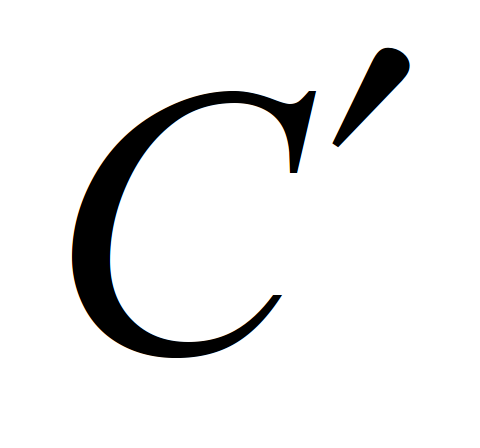
\includegraphics[width=0.252in,height=0.2398in]{crypt-img/crypt-img3.png} 
---отримана криптограма (\textit{C}\textit{ }може бути змінена при передачі,
наприклад, з-поза завад). Ключ \textit{k }заздалегідь передається по закритому
каналу одержувачу (або і відправнику, і одержувачу із джерела ключів), при
цьому неможливо отримати незаконному користувачу ніякої інформації щодо ключа,
здійснити будь-яку зміну в ключі  (вважається, що канал цілком надійний).
Призначення рандомізатора --- використовуючи  зовнішнє джерело випадковості
попередньо зрівняти деякі частотні характеристики ВТ.  Криптоаналітик завжди
може зчитувати ШТ з каналу передачі, але не може змінювати криптограми або мати
якийсь вплив на передачу ( так званий пасивний криптоаналітик).


\bigskip

{\centering \par}

\begin{figure}
\centering
\begin{minipage}{6.7165in}
{\centering 
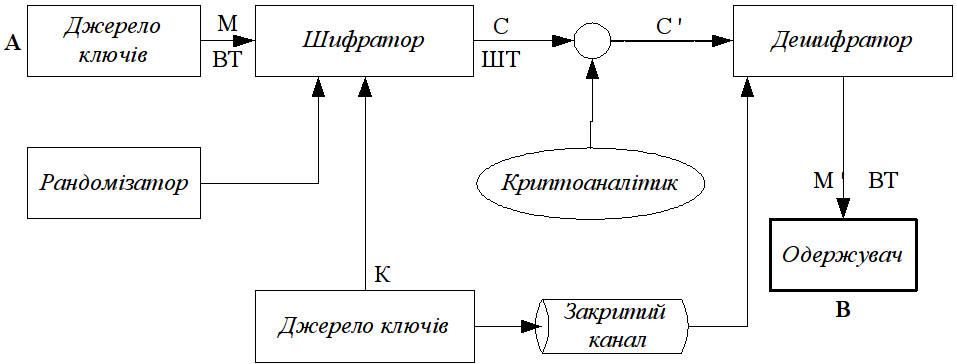
\includegraphics[width=6.5909in,height=2.5602in]{crypt-img/crypt-img4.png}
\par}
\begin{minipage}{1.1161in}
{\itshape
Відправник}
\end{minipage}\end{minipage}
\end{figure}
{\centering
\textbf{Рис 3.1.} \textit{Загальна схема секретного зв{\textquotesingle}язку.}
\par}


\bigskip

З математичної точки зору криптосистема є сукупністю просторів (множин)  ${\sum
?\{\text{M,K,C,E,D}\}}$,  де 

\textbf{М}--- простір всіх повідомлень; $ $

 
\includegraphics[width=0.2311in,height=0.2311in]{crypt-img/crypt-img5.png}  ---
простір ключів;

\textbf{С}--- простір криптограм;

\textbf{Е}--- простір алгоритмів шифрування;

\textbf{D}--- простір алгоритмів розшифрування.

Розглянемо  $M,X\in M$ --- деякі повідомлення, звичайно повідомлення --- це
послідовність букв  деякого алфавіту: 
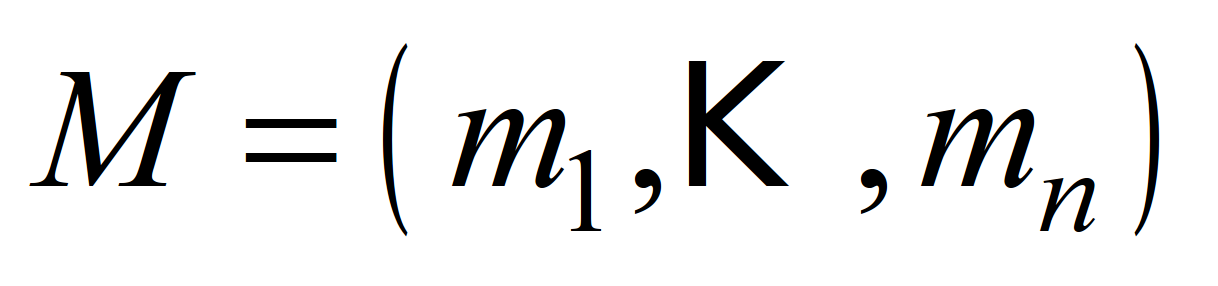
\includegraphics[width=1.311in,height=0.3189in]{crypt-img/crypt-img6.png} , 
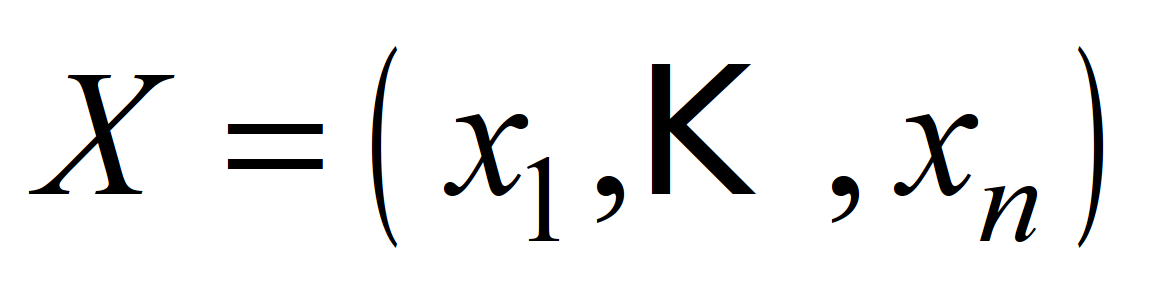
\includegraphics[width=1.2681in,height=0.3354in]{crypt-img/crypt-img7.png} , 
$m_i,x_j-$ символи ВТ, що є буквами відповідного алфавіту; 
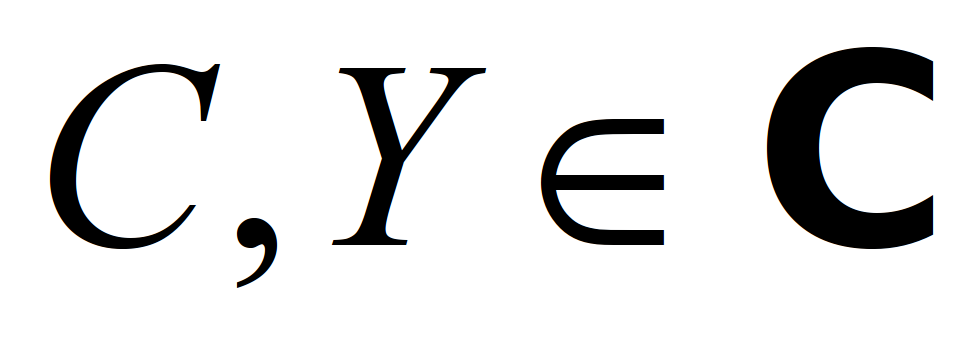
\includegraphics[width=0.739in,height=0.2709in]{crypt-img/crypt-img8.png}  ---
криптограми, що теж є, як правило, послідовністю символів деякого алфавіту; 
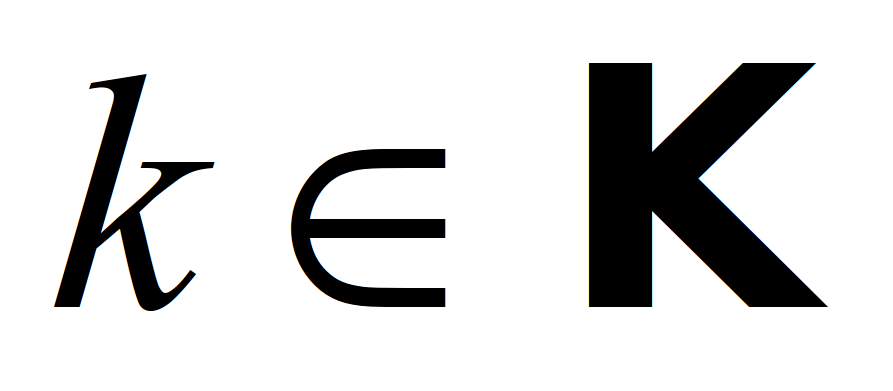
\includegraphics[width=0.5193in,height=0.2311in]{crypt-img/crypt-img9.png}  ---
деякий ключ; 
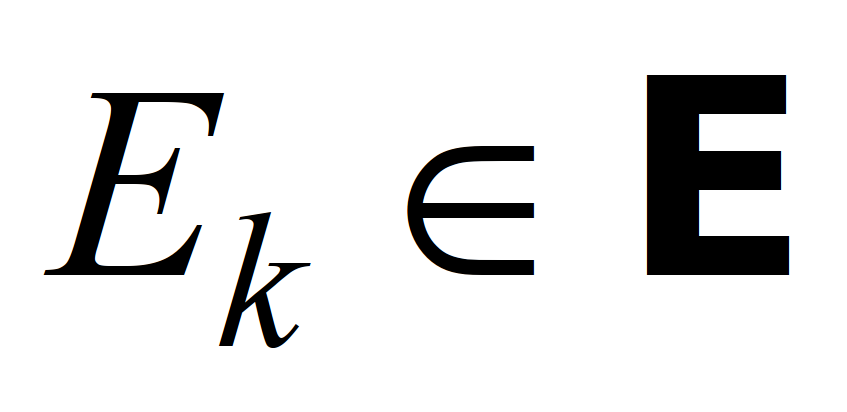
\includegraphics[width=0.6146in,height=0.3016in]{crypt-img/crypt-img10.png} , 
$D_k\in ?$ \textbf{D} --- конкретні перетворення (алгоритми) зашифрування і
розшифрування відповідно з ключем \textit{k}. 

У загальному випадку шифр --- це відображення \textbf{М} $?$

\includegraphics[width=0.2311in,height=0.2311in]{crypt-img/crypt-img11.png} 
$\rightarrow $\textbf{ С}, причому
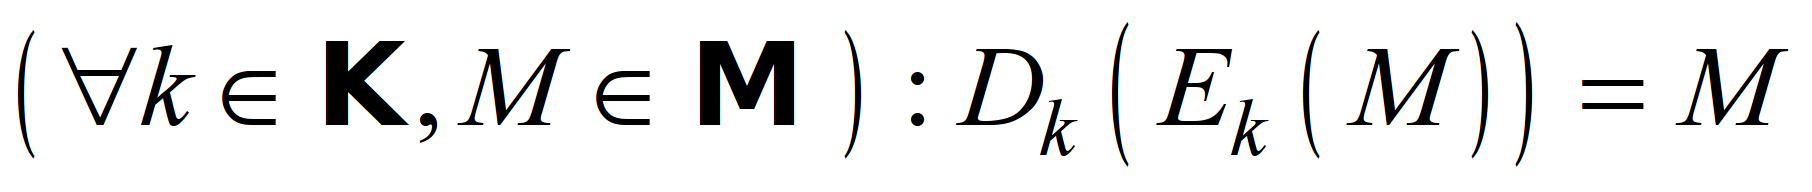
\includegraphics[width=3.1173in,height=0.3346in]{crypt-img/crypt-img12.png} , 
де   $E_k:$ \textbfМ $\rightarrow $\textbf{ С}
---ін{\textquotesingle}єктивне відображення, що дає можливість зашифрувати 
будь-який ВТ на ключі \textit{k.}

В теорії \textit{Шеннона} сформульовані наступні \textit{припущення}:

\liststyleWWviiiNumxix
\begin{enumerate}
\item Криптоаналітику відомий тільки шифрований текст, тобто атака здійснюється
на основі шифротексту.
\item Ключ і рандомізатор використовуються для шифрування тільки один раз (тобто
криптоаналіз здійснюється тільки по одній криптограмі). 
\item На  декартовому добутку  $M\times K$ задано ймовірнісний розподіл.
\end{enumerate}
 Цей список може бути доповнений новими припущеннями, які Шеннон використовував
неявно, зокрема, такими:  канал передачі без спотворень, перетворення
інформації без помилок, відсутній зворотний зв’язок. Хоча вже розроблені більш
загальні теорії, результати Шеннона заклали наріжний камінь криптографії як
науки.

 Згідно з правилом Керкгоффса  всі простори криптосистеми   $\Sigma $ $ $ та
розподіл на  М $?$ K  вважаються відомими криптоаналітику.


\bigskip

Нехай 
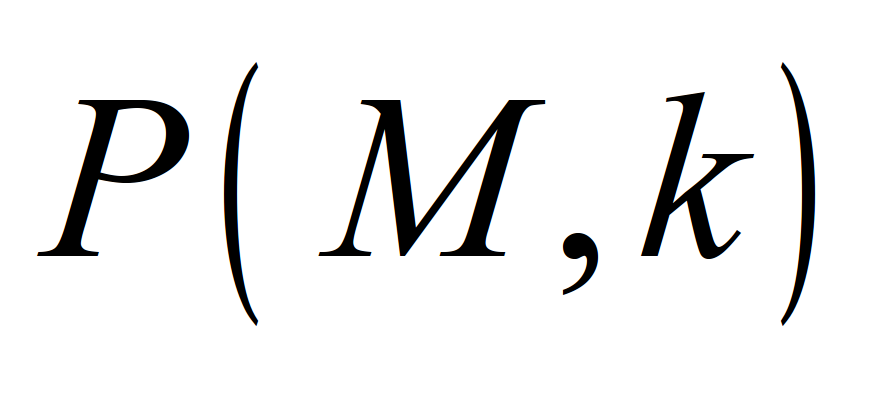
\includegraphics[width=0.7437in,height=0.3339in]{crypt-img/crypt-img13.png} , 
$\underset{M,k}{\sum }{P(M,k)=1}$  --- розподіл імовірностей на декартовому
добутку  $M\times K$. Зокрема, якщо відкритий текст і ключ, що генеруються,
незалежні (а частіше всього саме так на практиці), то 
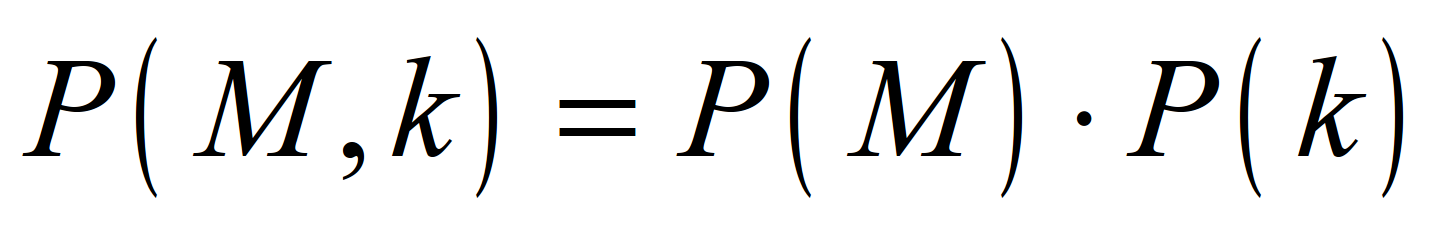
\includegraphics[width=1.9992in,height=0.3346in]{crypt-img/crypt-img14.png} .
Цей розподіл 
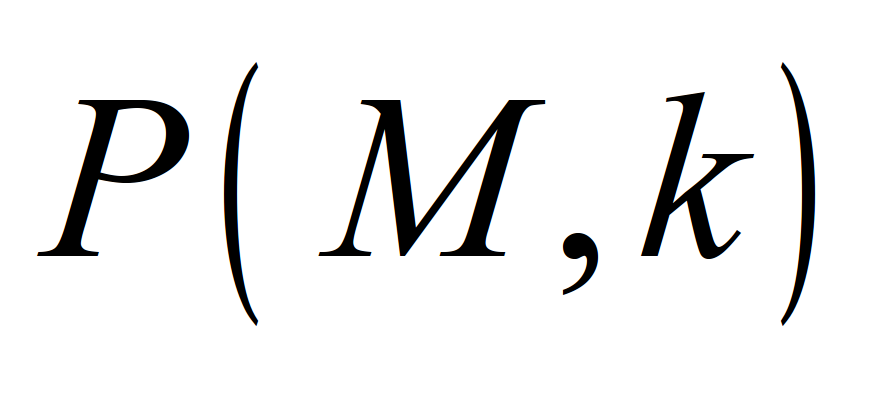
\includegraphics[width=0.7437in,height=0.3339in]{crypt-img/crypt-img15.png}  
індукує розподіли ймовірностей на інших множинах системи.  На просторах
алгоритмів шифрування Е, алгоритмів розшифрування  D та просторі  криптограм 
\textbf{С}  розподіли задаються формулами:

{\centering
 $\forall (k)$  
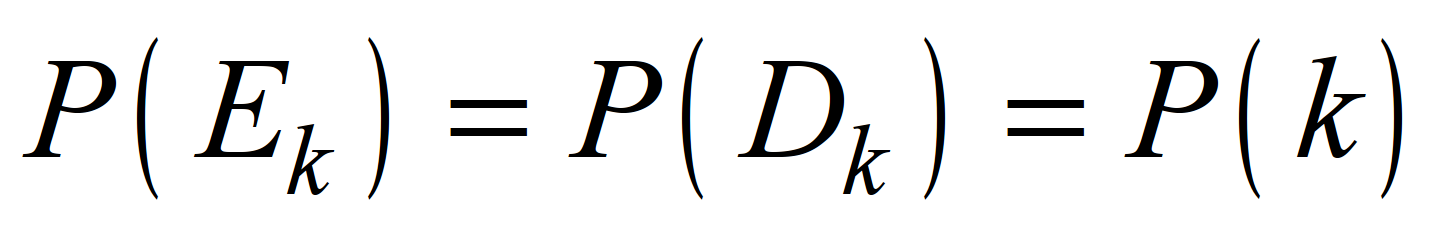
\includegraphics[width=1.9898in,height=0.3335in]{crypt-img/crypt-img16.png} ;
\par}

{\centering
 $\forall (C)$   
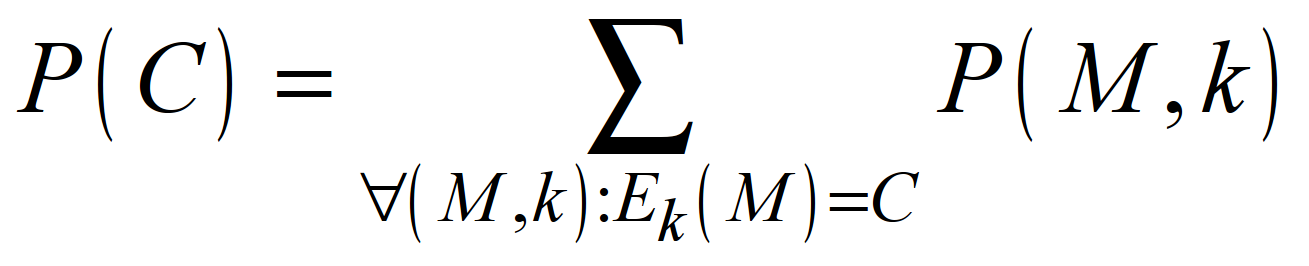
\includegraphics[width=2.5583in,height=0.5154in]{crypt-img/crypt-img17.png} ,
\par}

де останнє підсумовування здійснюється по всіх парах
(\textit{M},\textit{k}),\textit{ }для яких  $E_k(M)=C$.

Сумісний розподіл ймовірностей  криптограм і ключів  на \textbf{С} $?$
\textbf{К} задається формулою:

{\centering
 $\forall (C,k)$    
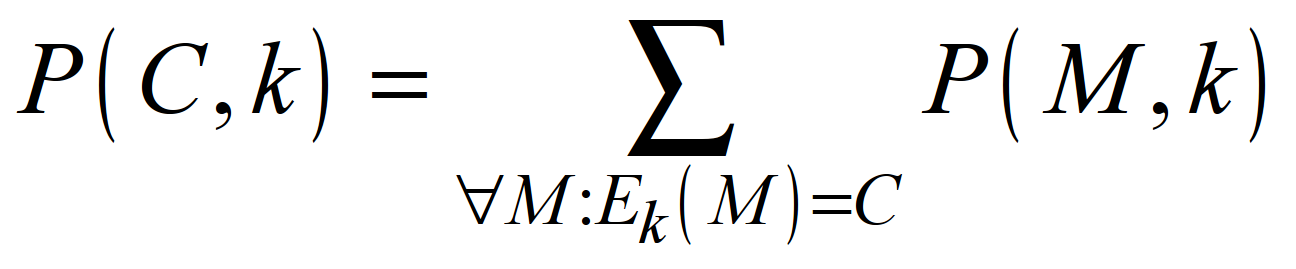
\includegraphics[width=2.5201in,height=0.5209in]{crypt-img/crypt-img18.png} .
\par}

Сумісний розподіл ймовірностей  криптограм і відкритих текстів на  \textbf{С}
$?$ \textbf{М}  індукується наступними співвідношеннями:


\bigskip

{\centering
 $\forall (C,M)$   
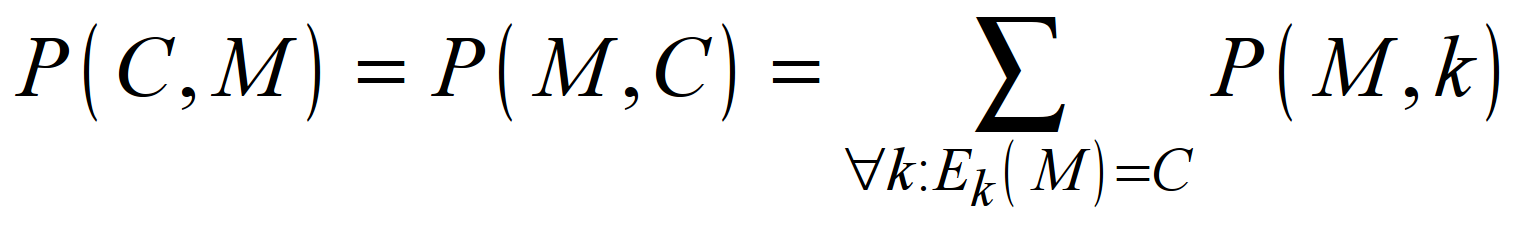
\includegraphics[width=3.478in,height=0.5209in]{crypt-img/crypt-img19.png} ;
\par}

Ймовірнісні розподіли на вказаних декартових добутках дають можливість знайти
умовні розподіли:

{\centering
 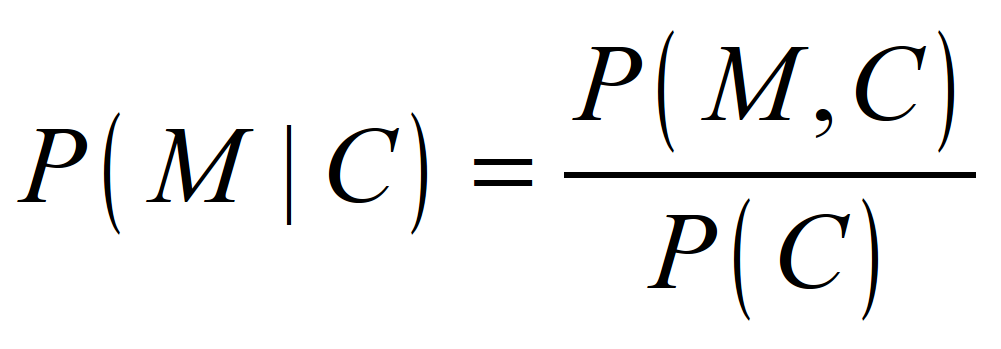
\includegraphics[width=1.7902in,height=0.6354in]{crypt-img/crypt-img20.png} ,  
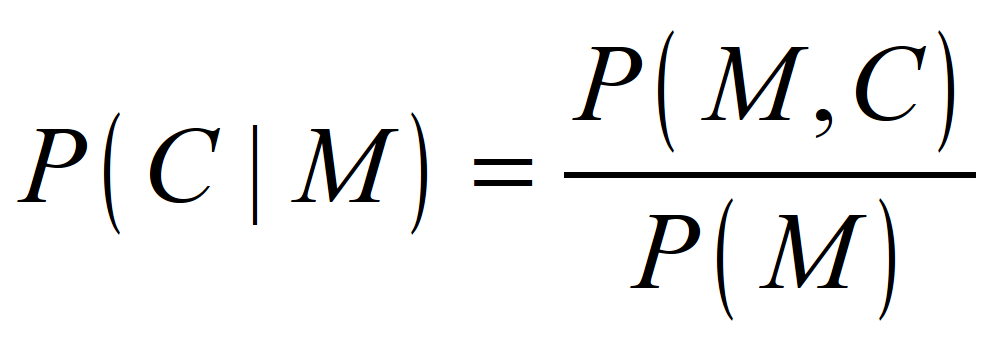
\includegraphics[width=1.7874in,height=0.6335in]{crypt-img/crypt-img21.png} ,  
$P(k/C)=\frac{P(k,C)}{P(C)}$.
\par}


\bigskip


\bigskip

\section{Цілком таємна (секретна)  криптосистема. Теореми  Шеннона.}


\bigskip


\bigskip

Після побудови вищезазначених розподілів можна розглядати також  ентропію множин
з ймовірнісною мірою і побудувати математичну модель криптосистеми. Поняття
цілком таємної криптосистеми формалізує властивість теоретичної стійкості у
теоретико-інформаційному розумінні.


\bigskip

$\blacklozenge$ О\textit{ЗНАЧЕННЯ}. Цілком таємною криптосистемою 

\includegraphics[width=0.1882in,height=0.2008in]{crypt-img/crypt-img22.png} 
називається криптосистема, для якої виконується одна з умов:

\liststyleWWviiiNumxliii
\begin{enumerate}
\item 
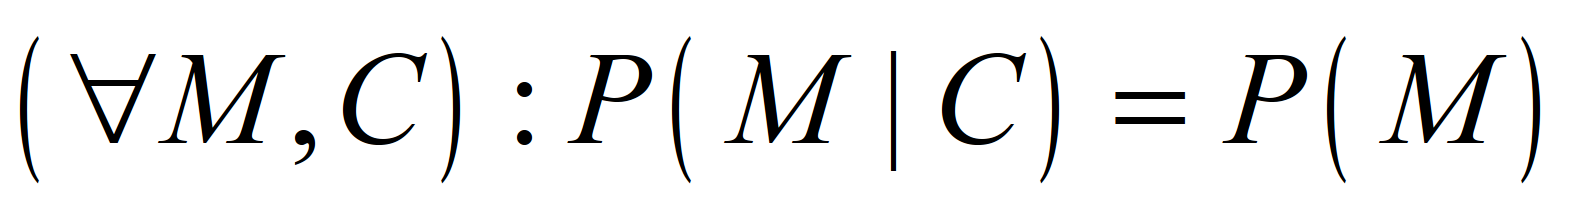
\includegraphics[width=2.3417in,height=0.3346in]{crypt-img/crypt-img23.png} ;
\item  \textit{H}\textit{ }( \textbf{M} {\textbar} \textbf{С}
)\textit{=}\textit{H}\textit{ }( \textbf{M} ), 
\end{enumerate}
де  \textit{H} \textbf{( }\textbf{M} )  і  \textit{H} (  \textbf{M}\textbf{
{\textbar} С} ) --- ентропія і  умовна ентропія відповідно.

\liststyleWWviiiNumxliii
\setcounter{saveenum}{\value{enumi}}
\begin{enumerate}
\setcounter{enumi}{\value{saveenum}}
\item \textbf{\textit{Зауваження}}\textbf{.} Умови 1 і 2 еквівалентні, з
виконанням  однієї умови буде виконуватись і інша. Умова 1 означає, що ВТ і ШТ
статистично незалежні. Умову 2 можна інтерпретувати як відсутність в ШТ
інформації відносно ВТ, тобто взаємна інформація  
\end{enumerate}
\textit{ } \textit{I}\textit{
}\textbf{(}\textbf{M}\textbf{,}\textbf{C}\textbf{)}=\textit{ H}( \textbf{M} ) ---
\textit{H}(\textbf{M} {\textbar} \textbf{С)=0}


\bigskip

\textit{ТЕОРЕМА 3.1 }Необхідною і достатньою умовою цілковитої секретності
криптосистеми є виконання будь-якої  з умов:

\liststyleWWviiiNumxi
\begin{enumerate}
\item 
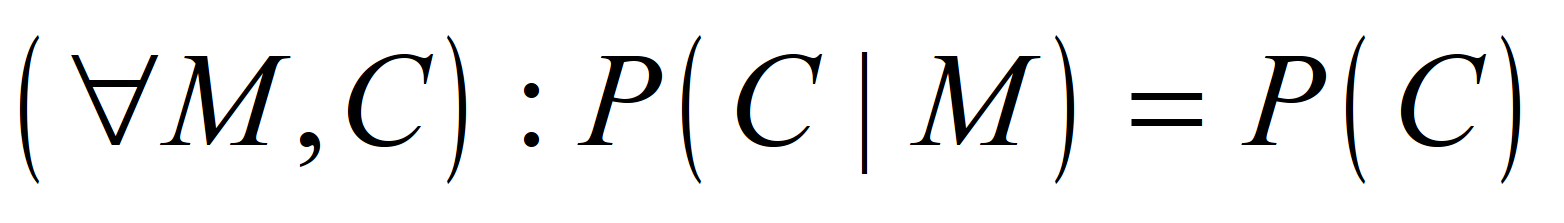
\includegraphics[width=2.3146in,height=0.3346in]{crypt-img/crypt-img24.png} ;
\item \textit{ H }( \textbf{С}\textbf{ {\textbar} }\textbf{М} )\textit{=H }(
\textbf{С }) .
\end{enumerate}
\textlatin{[F034?]}\textit{Необхідність}. Якщо система цілком таємна, то 
$P(M)=P(M|C)=\frac{P(M,C)}{P(C)}$  $ $ $ $ $\Rightarrow$ 
$\frac{P(M,C)}{P(M)}=P(C)=P(C|M)$ .  Аналогічно доводиться
\textit{достатність}.\textlatin{[F033?]}


\bigskip

Виникає питання: чи існують цілком таємні криптосистеми? \textit{Розглянемо
такий приклад}. Шифр Вернама (1926 р.). Відкритий текст кодується двійковою
послідовністю, ключ та шифртекст  також представляються послідовностями  „0” і
„1” такої ж довжини. ШТ отримується з ВТ і ключа операцією XOR.


\bigskip

 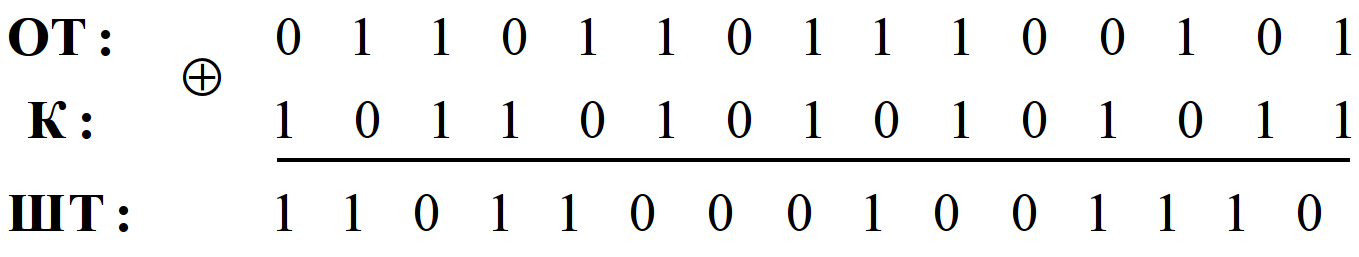
\includegraphics[width=4.111in,height=0.778in]{crypt-img/crypt-img25.png} 


\bigskip

У якості ключа береться «ідеально» випадкова послідовність --- послідовність
незалежних рівноймовірних випадкових біт, тобто кожна реалізація довжини 
\textit{n }з‘являється з ймовірністю  $2^{-n}$ незалежно від ВТ. У даному
прикладі ймовірність появи будь-якої ключової послідовності, а також будь-якої
криптограми  
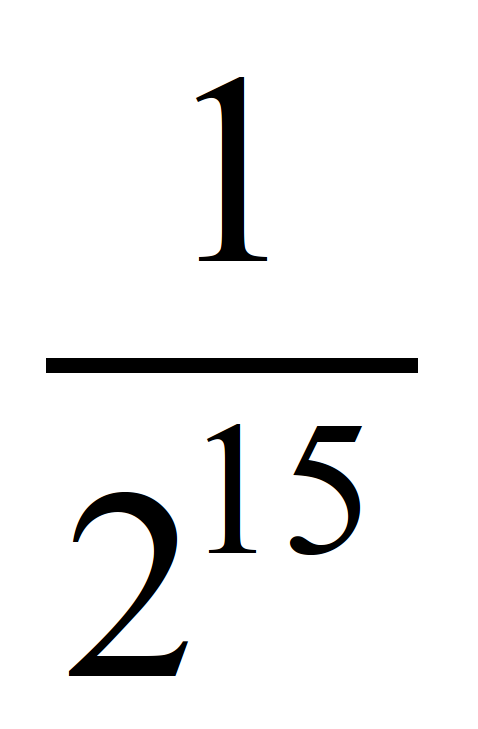
\includegraphics[width=0.2917in,height=0.4437in]{crypt-img/crypt-img26.png} .

Даний шифр застосовується дотепер (так звана стрічка одноразового користування
або одноразовий блокнот) на окремих важливих напрямах зв’язку. За допомогою
побудованої теорії Шеннон  довів, що цей шифр  є цілком таємним, тобто маючи
тільки криптограму  ніяким чином не можливо знайти відкритий текст і навіть
будь-яку інформацію щодо нього. Головним недоліком шифра Вернама є велика
довжина ключа, що треба попередньо передавати по закритому каналу. 


\bigskip

\textit{ТЕОРЕМА }\textit{3}\textit{.2  }Шифр Вернама є цілком таємною
криптосистемою.

\textlatin{[F034?]} \textit{Доведення}. Маємо відкритий текст: 
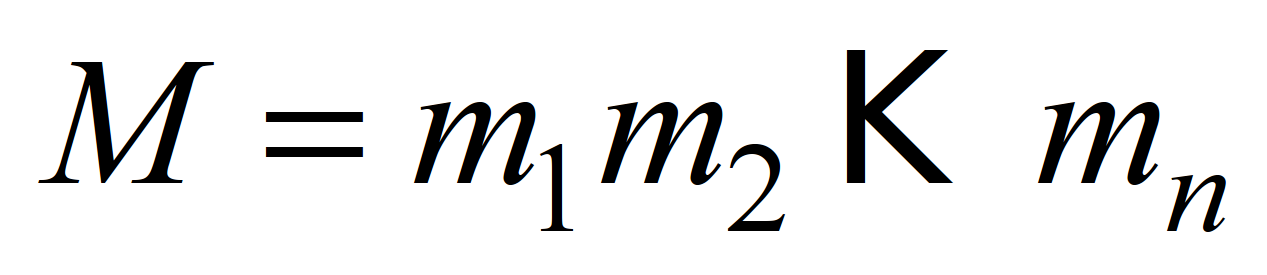
\includegraphics[width=1.2591in,height=0.2709in]{crypt-img/crypt-img27.png} ,
ключ: 
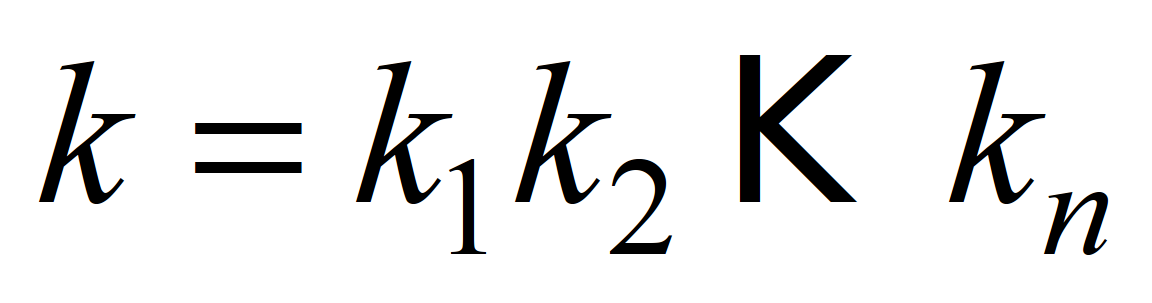
\includegraphics[width=1.0827in,height=0.2791in]{crypt-img/crypt-img28.png} ,
криптограму: 
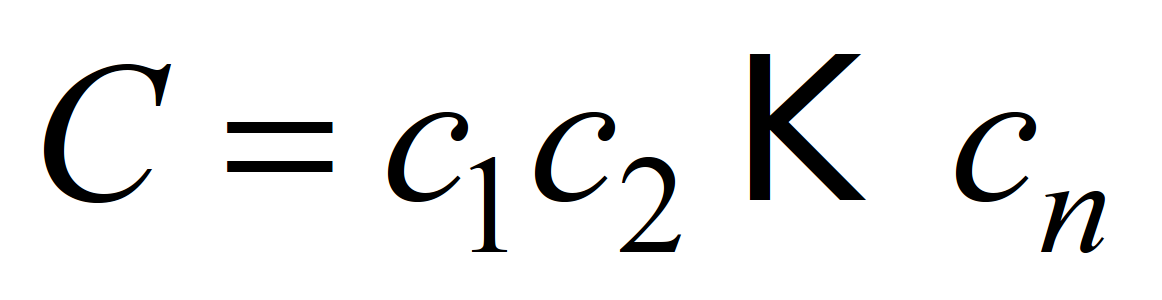
\includegraphics[width=1.2283in,height=0.3146in]{crypt-img/crypt-img29.png} , 
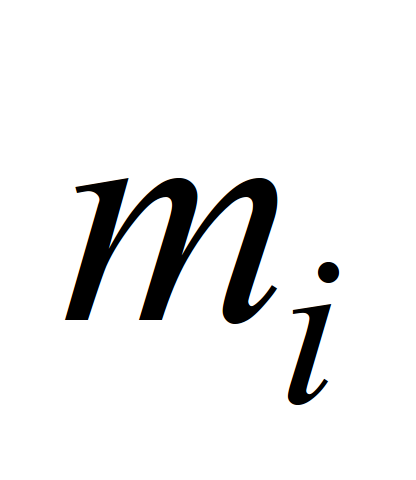
\includegraphics[width=0.2591in,height=0.3063in]{crypt-img/crypt-img30.png} , 
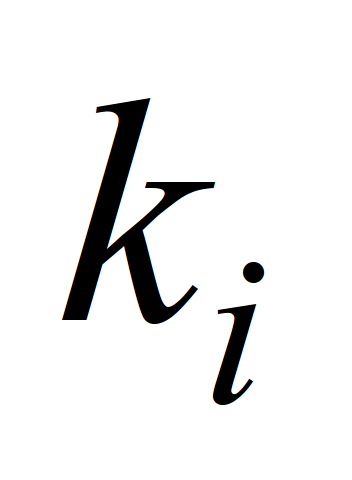
\includegraphics[width=0.2402in,height=0.3118in]{crypt-img/crypt-img31.png} , 
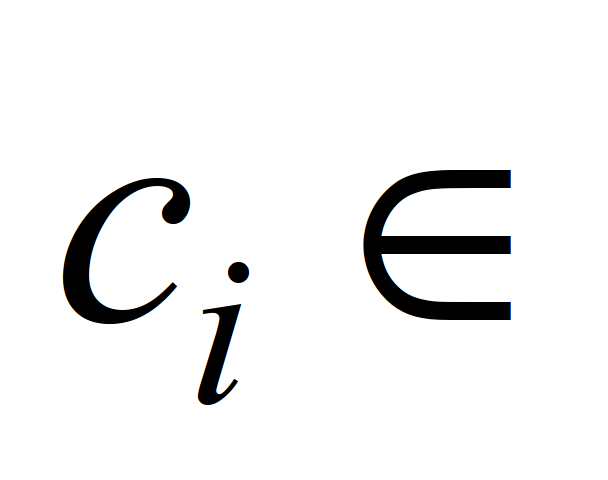
\includegraphics[width=0.3929in,height=0.3126in]{crypt-img/crypt-img32.png} 
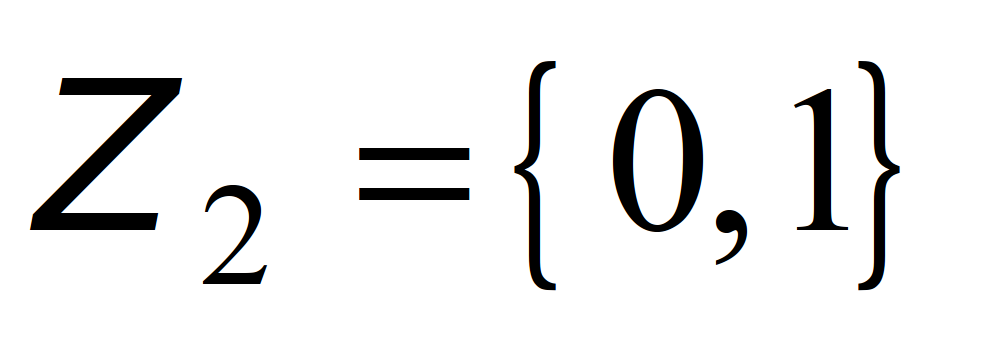
\includegraphics[width=0.9835in,height=0.3547in]{crypt-img/crypt-img33.png} ;

 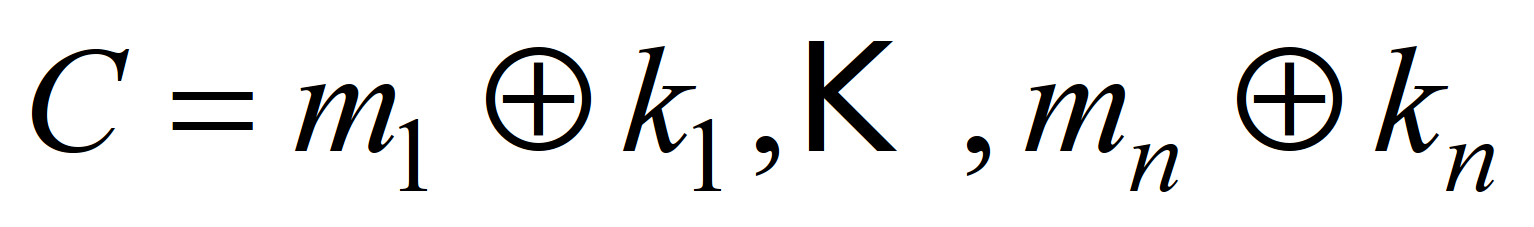
\includegraphics[width=1.8819in,height=0.2791in]{crypt-img/crypt-img34.png} . 
Використовуємо теорему 2.1. Безпосередньо знаходимо, що ймовірність появи
будь-якої криптограми дорівнює:

{\centering
 $\forall (C)$  
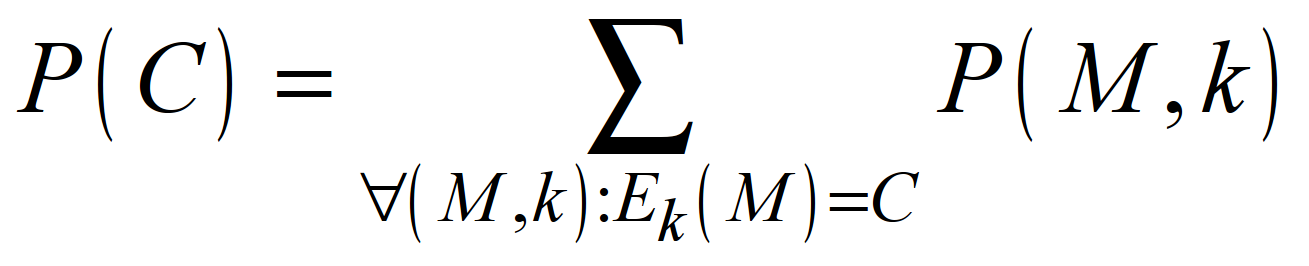
\includegraphics[width=2.5984in,height=0.5189in]{crypt-img/crypt-img35.png} =
$2^{-n}\undersetM{\sum }{P(M)}=2^{-n}$,
\par}

{\centering
тому що
\textit{P}\textit{(}\textit{M}\textit{,}\textit{k}\textit{)=}\textit{P}\textit{(}\textit{M}\textit{)}\textit{P}\textit{(}\textit{k}\textit{)=}
$2^{-n}$ \textit{P}\textit{(}\textit{M}\textit{)},  а  умовна ймовірність: 
$\forall (C,M)$  
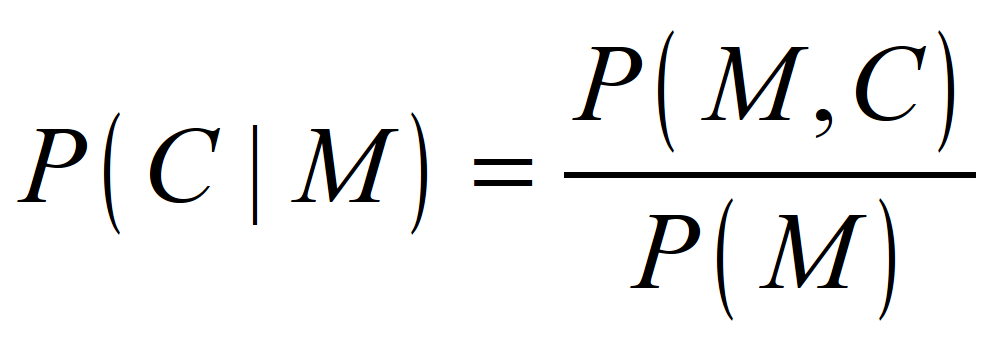
\includegraphics[width=1.8862in,height=0.661in]{crypt-img/crypt-img36.png} ,  
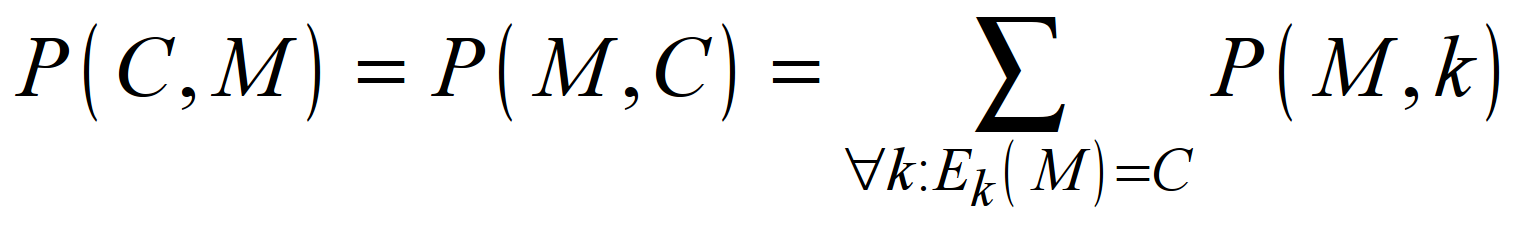
\includegraphics[width=3.602in,height=0.539in]{crypt-img/crypt-img37.png} 
Звідки  $\Rightarrow P(C|M)=P(M)2^{-n}/P(M)=2^{-n}$. 
\par}

Таким чином, згідно з теоремою 3.1, шифр Вернама --- цілком таємна криптосистема.


\bigskip

\textit{ТЕОРЕМА }\textit{3}\textit{.3 (Шеннон)} Якщо криптосистема цілком
таємна, то  $H(M)\le H(K)$. Ця нерівність називається межею Шеннона.

\textlatin{[F034?]}\textit{Доведення.} Оскільки система цілком таємна, то 

\begin{equation*}
\begin{matrix}{H(M)=H(M|C)\le H(\normalsubformula{\text{M,K}}|C)=}\hfill\null
\\{=H(K|C)+H(M|\normalsubformula{\text{K,C}})=H(K|C)\le H({K})}\hfill\null
\end{matrix}\hfill 
\end{equation*}
Тут   $H(M|K,C)=0$, бо при відомих ШТ і  ключах ВТ однозначно відновлюється. 
Таким чином,   $H(M)\le H(K)$.\textlatin{[F033?]}

\textit{Зауваження.} Границя (нерівність) Шеннона є необхідною, але не
достатньою умовою цілковитої таємності криптосистеми.

Якщо ключі вибираються рівноймовірно, то ентропія ключів максимальна і дорівнює
довжині ключа в бітах (даного двійковою послідовністю). Для розумного тексту
природною мовою заданого у двійковому алфавіті ентропія дорівнює приблизно
чверті його довжині в бітах. Якби надлишковість дорівнювала нулю, ентропія
такого тексту співпадала б з числом двійкових символів у ньому (дивись лекцію
2). З теореми 2.3 випливає, що у цілком таємної системи при шифруванні тексту
великого розміру таємний ключ теж повинен бути великого розміру (довжини, якщо
задається послідовністю символів). І при зростанні обсягу тексту розмір ключа
повинен зростати пропорційно. Таким чином, криптосистема з фіксованим ключем в
загальному випадку не може бути цілком таємною. Для цілковитої таємності
секретні ключі для більшості практичних застосувань мають бути занадто
великими. Тому майже усі криптосистеми, що використовуються на практиці загалом
не є цілком таємними. Вони не мають теоретичної стійкості в
теоретико-інформаційному сенсі й  у принципі можуть бути зламані. Для таких
криптосистем характеристикою їх надійності є практична стійкість. Для не цілком
таємних систем Шеннон розглянув питання теоретико-інформаційної ненадійності, а
також необхідного для зламу шифру обсягу криптограми ( це --- тема наступної
лекції).


\bigskip

\section{Контрольні питання}


\bigskip


\bigskip

\liststyleWWviiiNumxlv
\begin{enumerate}
\item Чим відрізняються процедури зашифрування та розшифрування?
\item Як визначається поняття теоретичної та практичної стійкості криптосистеми?
\item Сформулюйте правило Керкгоффса.
\item Які припущення зробив Шеннон у запропонованій ним моделі випадкового
шифру?
\item Наведіть означення цілком таємної системи в теорії Шеннона.
\item Що таке границя Шеннона?
\item Чи виконання нерівності Шеннона є достатньою умовою для цілковитої
таємності?
\item Чи існують цілком таємні криптосистеми? 
\end{enumerate}

\bigskip


\bigskip


\bigskip

 $ $\textbf{ ЛЕКЦІЯ  4}


\bigskip

{\centering\bfseries
НЕНАДІЙНІСТЬ  КЛЮЧА  І  ВІДКРИТОГО  ТЕКСТУ.
\par}

{\centering\bfseries
 ВІДСТАНЬ  ОДНОЗНАЧНОСТІ
\par}


\bigskip


\bigskip

Для цілком таємної криптосистеми неможливо з криптограми здобути будь-яку
інформацію щодо відкритого тексту. Якщо ж криптосистема не є цілком таємною (а
більшість криптосистем, що використовуються на практиці, саме такі), то за
криптограмою  можна отримати певну інформацію про текст, що був зашифрований,
про таємний ключ, а можливо повністю зламати шифр --- знайти таємний ключ і
відкритий текст. Розглянемо ці питання докладніше.


\bigskip

\textit{Означення4.1}.  \textit{Ненадійністю ключа }називається  величина 

{\centering
  $H(K|C)=-\underset{K,C}{\sum }{P(K,C)\textlogP(K|C)}$.
\par}

\textit{Означення4.2}\textit{. Ненадійністю відкритого }\textit{тексту}
називається  величина 

{\centering
 $H(M|C)=-\underset{M,C}{\sum }{P(M,C)\textlogP(M|C)}$. $ $
\par}

Тобто  криптограма  містить у середньому \textit{I}\textit{
}\textbf{(}\textbf{M}\textbf{,}\textbf{C}\textbf{)}=\textit{
}\textit{H}\textbf{(}\textbf{M}\textbf{) -
}\textit{H}(\textbf{M}\textbf{/}\textbf{C}\textbf{)}\textbf{  }біт\textbf{
}інформації відносно ВТ (у цілком таємної криптосистеми така інформація
дорівнює нулю) і  \textit{I}\textit{
}\textbf{(}\textbf{K}\textbf{,}\textbf{C}\textbf{)}=\textit{
}\textit{H}\textbf{(}\textbf{K}\textbf{)-}\textit{
}\textit{H}\textbf{(}\textbf{K}\textbf{/}\textbf{C}\textbf{)}\textbf{ }біт
інформації щодо ключа. 

\textit{ТЕОРЕМА 4.1}\textit{  }Нехай в моделі криптосистеми за Шенноном  ( див.
лекцію \textbf{3})  ключ вибирається незалежно від ВТ. Тоді для ненадійності 
ключа буде виконуватись рівність  

{\centering
\textit{H}(\textbf{K}\textbf{/}\textbf{C}) =  \textit{H}(\textbf{M}) +
\textit{H}(\textbf{K}) \textit{--- }\textit{H}(\textbf{C}).
\par}

{\itshape
Доведення }

\textit{ }Згідно\textit{ }з властивостями умовної ентропії 

\textit{H}\textbf{(}\textbf{M}\textbf{,}\textbf{K}\textbf{,}\textbf{C}\textbf{)
= }\textit{H}\textbf{(}\textbf{M}\textbf{,}\textbf{K}\textbf{) }\textit{+
}\textit{H}\textbf{(}\textbf{C}\textbf{/}\textbf{M}\textbf{,}\textbf{K}\textbf{)
= }\textit{H}\textbf{(}\textbf{K}\textbf{,}\textbf{C}\textbf{) }\textit{+
}\textit{H}\textit{(}\textbf{M}\textbf{/}\textbf{K}\textbf{,}\textbf{C}\textbf{).
}

\textbf{О}скільки через однозначність шифрування та розшифрування 
\textit{H}\textbf{(}\textbf{C}\textbf{/}\textbf{M}\textbf{,}\textbf{K}\textbf{)
=}\textit{H}\textbf{(}\textbf{M}\textbf{/}\textbf{K}\textbf{,}\textbf{C}\textbf{)=}0\textbf{,
}то\textbf{
}\textit{H}\textbf{(}\textbf{K}\textbf{,}\textbf{C}\textbf{)=}\textit{H}\textbf{(}\textbf{M}\textbf{,}\textbf{K}\textbf{)}\textbf{.}\textbf{
}

Далі, враховуючи незалежність ключів і ВТ, отримуємо  \textbf{ }

\textit{H}\textbf{(}\textbf{M}\textbf{,}\textbf{K}\textbf{) =
}\textit{H}\textbf{(}\textbf{M}\textbf{) +
}\textit{H}\textbf{(}\textbf{K}\textbf{) } $\Rightarrow $\textit{
}\textit{H}\textbf{(}\textbf{K}\textbf{,}\textbf{C}\textbf{) =
}\textit{H}\textbf{(}\textbf{M}\textbf{) +
}\textit{H}\textbf{(}\textbf{K}\textbf{)}. З іншого боку

\textit{H}\textbf{(}\textbf{K}\textbf{,}\textbf{C}\textbf{) }\textit{=
}\textit{H}\textbf{(}\textbf{C}\textbf{) +
}\textit{H}\textbf{(}\textbf{K}\textbf{/}\textbf{C}\textbf{) } ${\Rightarrow
}$\textbf{ }\textit{H}\textbf{(}\textbf{K}\textbf{/}\textbf{C}\textbf{) =
}\textit{H}\textbf{(}\textbf{M}\textbf{) +
}\textit{H}\textbf{(}\textbf{K}\textbf{) ---
}\textit{H}\textbf{(}\textbf{C}\textbf{)}.\textbf{ }Теорема\textbf{ }доведена.

Розглянемо модель Шеннона  криптосистеми  з незалежними  від відкритого тексту
ключами, в якої ВТ і ШТ --- це послідовності довжини  \textit{n}\textit{ }
символів з алфавіту   $Z_m$,  \textitn $?$\textit{
}\textbf{\textit{N}}\textit{.}  Причому,  ВТ --- розумний текст з середньою
інформацією на символ  $H_{\infty }$.  Позначимо  через   $ $   $ $ $ $ $ $
 \textbf{K}(C) =   ${\left\{\;k\in K:\exists
M,\;E_{k}\right.(M)=C\left.  \right\}}$

множину ключів, при шифруванні на яких  може бути отримано ШТ  \textit{С} (для
деяких повідомлень). Для фіксованого ШТ  \textit{С}  число хибних ключів
дорівнює   $|K(C)|-1$. Середнє число хибних ключів 


\bigskip

{\centering
\textit{k} $}_n$ =   $\underset{C\in C}{\sum }{P(C)\cdot (|K(C)|-1)$
=   $\underset{C\in C}{\sum }{P(C)|K(C)|-1}$
\par}


\bigskip

\textit{ТЕОРЕМА 4.2}\textit{  }Для будь-якого шифру   $\sum $ з незалежними
від ВТ ключами  при достатньо великих \textit{n} виконується  нерівність 

{\centering
\textit{k} $_n$   $?$  
$\frac{2^{H(K)}}{m^{\normalsubformula{\textnR}}}$ ---  1 
\par}


\bigskip

 де  \textit{R}  {}-  надлишковість  ВТ, що при достатньо великих \textit{n}
дорівнює надлишковості мови ВТ (див. лекцію 2).

{\itshape
Доведення }

 Для  достатньо великих  \textit{n} 

{\centering\bfseries
 $H($ M) ${?\normalsubformula{\text{nH}}_{\infty
}=\normalsubformula{\text{nH}}_{0}(1-R)=n(\log _{2}m)(1-R)\text{.}}$
\par}

Очевидно \textit{ }\textit{H}(\textbf{C})  $?$  log $_2$
$|\text{С}|$ =  \textit{n} log $_2$ \textit{m}\textit{.}  З останніх
двох співвідношень та теореми 4.1  отримуємо:

{\centering
\textit{H}(\textbf{K}\textbf{/}\textbf{C}) = \textit{H}(\textbf{M}) +
\textit{H}\textit{(}\textbf{K}) --- \textit{H}(\textbf{C})  $?$ 
\textit{H}(\textbf{K}) + \textit{n} (log $_2$ \textit{m})
(1-\textit{R}) ---
\par}

{\centering
--- \textit{H}(\textbf{C})  $?$ \textit{H}\textit{(}\textbf{K}) +
\textit{n}(1-\textit{R}) log $_2$ \textit{m} --- \textit{n} log
${}_2$ \textit{m} = \textit{H}(\textbf{K}) --- \textit{nR} log $_2$
\textit{m}.
\par}

Таким чином, 

{\centering
\textit{H}(\textbf{K}\textbf{/}\textbf{C}) $?$\textit{ }\textit{H}(\textbf{K})
--- \textit{n}\textit{ }\textit{R} log $_2$ \textit{m}.
\par}

З іншого боку маємо:

{\centering
\textit{H}(\textbf{K}\textbf{/}\textbf{C}) =   $\underset{C\in C}{\sum }$
\textit{P}(C) \textit{H}(\textbf{K}/\textit{C})  $?$  ${\underset{C\in
C}{\sum }{}}$ \textit{P}(\textit{C}) log $_2$ $|K(C)|$ .
\par}

Далі за нерівністю Ієнсена

{\centering
\textit{H}(\textbf{K}\textbf{/}\textbf{C})   $?$ log $_2$(
$\underset{C\in C}{\sum }$ \textitP(\textitC\textbf{) } $|K(C)|$ = 
log ${}_2$(\textit{k} $_n$+ 1) $ $
\par}

Враховуючи обидві отримані нерівності для 
\textit{H}(\textbf{K}\textbf{/}\textbf{C}) можемо тепер записати таку
нерівність 

{\centering
\textit{H}(\textbf{K}) --- \textit{n}\textit{ }\textit{R} log $_2$
\textit{m}   $?$  log ${}_2$(\textit{k} $_n$+1)
\par}

Звідки  маємо

{\centering
log  $\frac{2^{H(K)}}{m^{\normalsubformula{\textnR}}}$   $?$  log
(\textit{k} $_n$+1).
\par}

І  далі отримуємо твердження теореми 4.2:  \textit{k} $_n$   $?$  
$\frac{2^{H(K)}}{m^{\normalsubformula{\textnR}}}$  --- 1. 

Нехай 
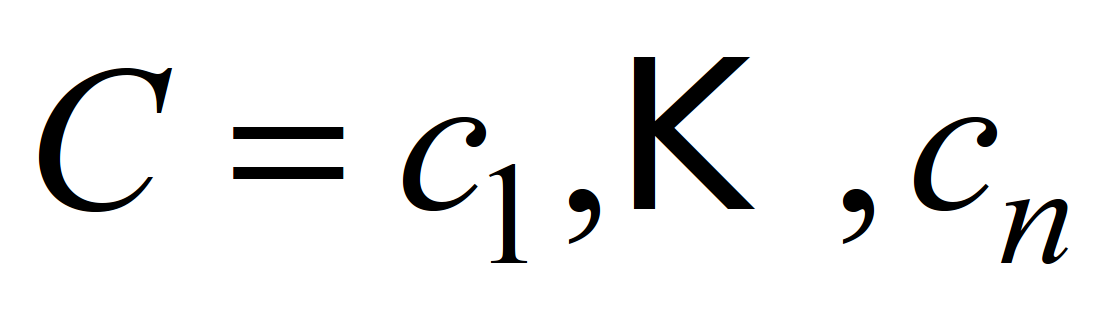
\includegraphics[width=1.1764in,height=0.3327in]{crypt-img/crypt-img38.png} ,  
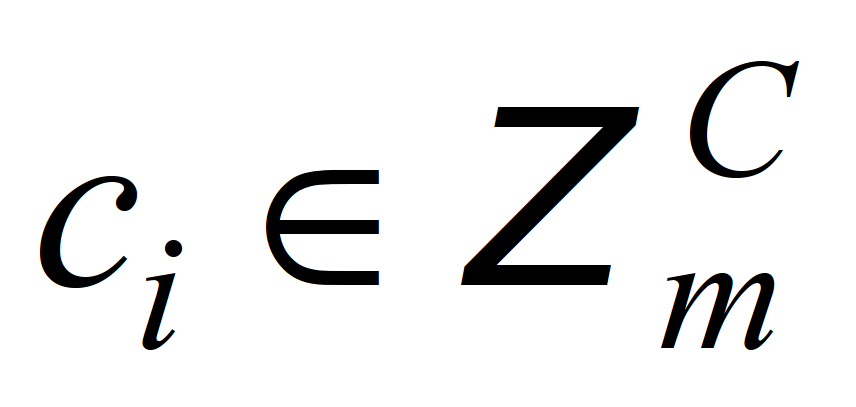
\includegraphics[width=0.7201in,height=0.3472in]{crypt-img/crypt-img39.png} , ---
деяка криптограма, 
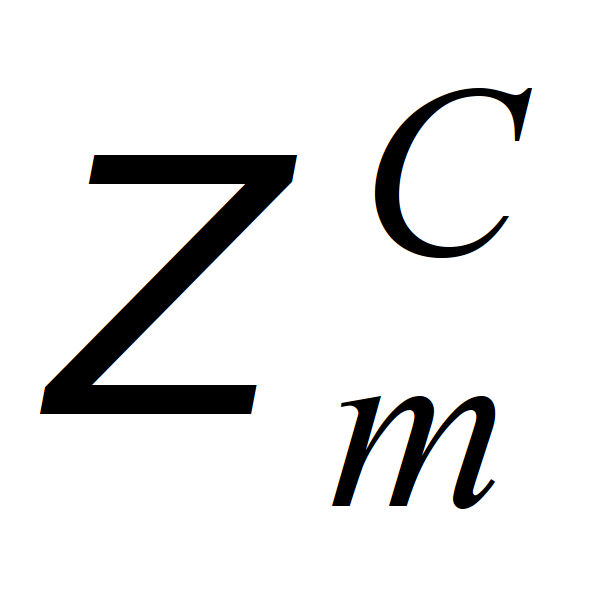
\includegraphics[width=0.3465in,height=0.3465in]{crypt-img/crypt-img40.png}  ---
алфавіт криптограм.

\textit{Означення 4.3}. \textit{Функцією ненадійності ключа} називається 
функція 

{\centering 
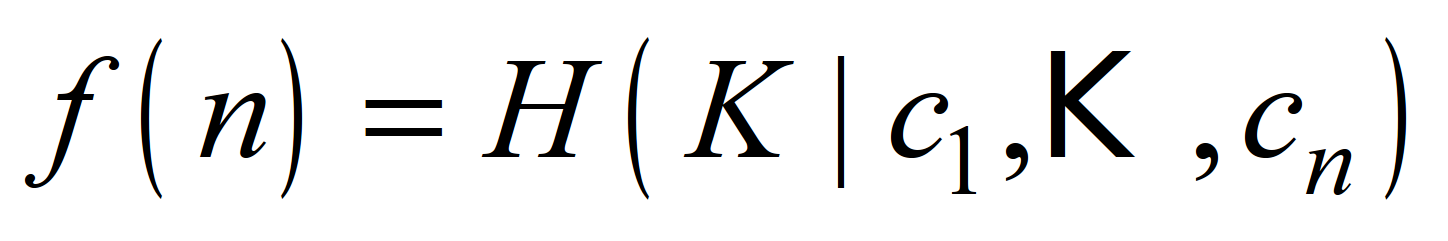
\includegraphics[width=1.9882in,height=0.3346in]{crypt-img/crypt-img41.png}
\par}

(ентропія ключа за умови, що відомо \textit{n }символів криптограми).

Очевидно, що 
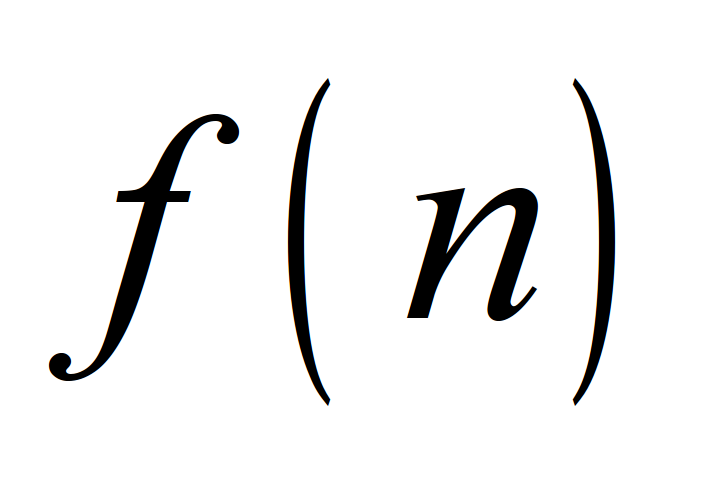
\includegraphics[width=0.4874in,height=0.3354in]{crypt-img/crypt-img42.png}  ---
незростаюча функція, а саме:

{\centering
 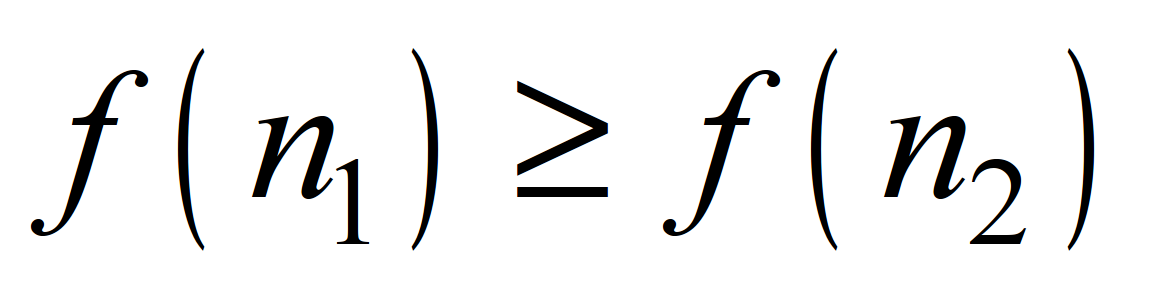
\includegraphics[width=1.2555in,height=0.3339in]{crypt-img/crypt-img43.png} , 
коли  
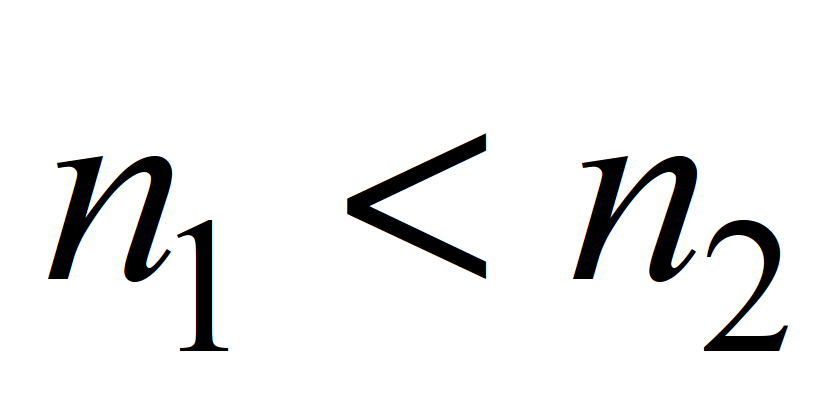
\includegraphics[width=0.598in,height=0.2984in]{crypt-img/crypt-img44.png} .
\par}

\textit{Означення4.4}. \textit{Відстанню  однозначності} називається
величина\textit{  } \textit{u}\textit{ }= min 
$\left\{ \;n|k_n \right.=0\left.  \right\}$

Тобто  за криптограмою довжиною більшою, ніж відстань однозначності,
криптоаналітик в принципі може знайти таємний ключ, що використовувався при
зашифруванні, оскільки його невизначеність дорівнює нулю. Але, як ми побачимо в
наступних лекціях, це не завжди можливо через  велику трудомісткість необхідних
обчислень. Зауважимо, що відстань однозначності --- це усереднена за ключами та
криптограмами (а отже і відкритими текстами) характеристика.

\textit{ТЕОРЕМА 4.3 } Для будь-якого шифру   $\sum $ з незалежними від ВТ 
ключами  при достатньо великих \textit{n} виконується  співвідношення

{\centering
\textit{u}\textit{ }=   $\frac{H(K)}{R\textlogm}$
\par}

{\itshape
Доведення}

 Таємний ключ може бути однозначно знайдений за  криптограмою, якщо число хибних
ключів дорівнює нулю. Тобто, з урахуванням усереднення за ключами і
криптограмами, це означає, що\textit{  }\textit{k} $_n$=0. Далі з
теореми 4.2 отримаємо: 

{\centering
1   $?$   $\frac{2^{H(K)}}{m^{\normalsubformula{\textnR}}}$  
$\Rightarrow $\textit{  }\textit{n}\textit{ }\textit{R}\textit{ }log
\textit{m}  $?$  \textit{H}(\textbf{K}) 
\par}


\bigskip

Звідки  випливає, що  \textit{n}  $?$  \textit{H}(\textbf{K}) / \textit{R} log
\textit{m}\textit{.}\textit{ }З останньої нерівності видно, що мінімальне
\textit{n}, для якого середнє число хибних ключів дорівнює нулю, задається
формулою для відстані однозначності, що наведена у формулюванні теореми.   $ $
$ $ 

Формула Шеннона для відстані однозначності добре погоджується з криптографічною
практикою при достатній довжині криптограми  і у більш загальних випадках

{\itshape
 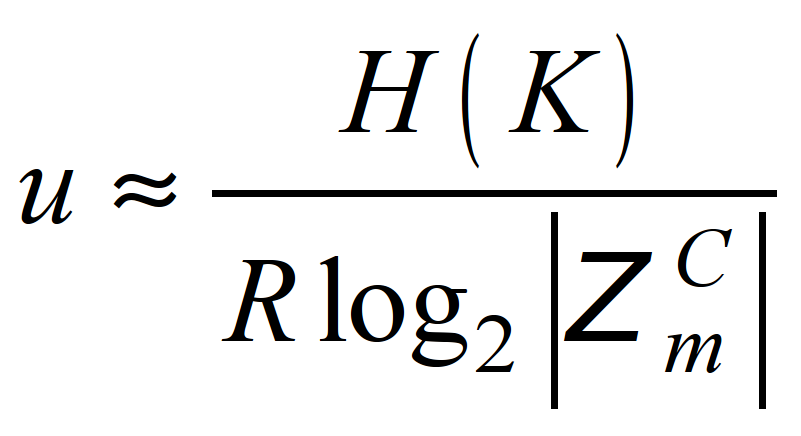
\includegraphics[width=1.3335in,height=0.7189in]{crypt-img/crypt-img45.png} ,}

де \textit{R}\textit{ }--- надлишковість криптограми,  

{\centering
 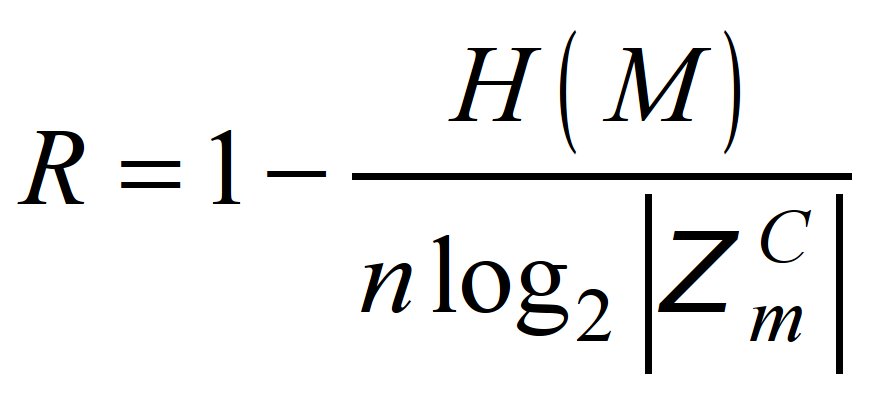
\includegraphics[width=1.5626in,height=0.7118in]{crypt-img/crypt-img46.png} .
\par}

Запис 
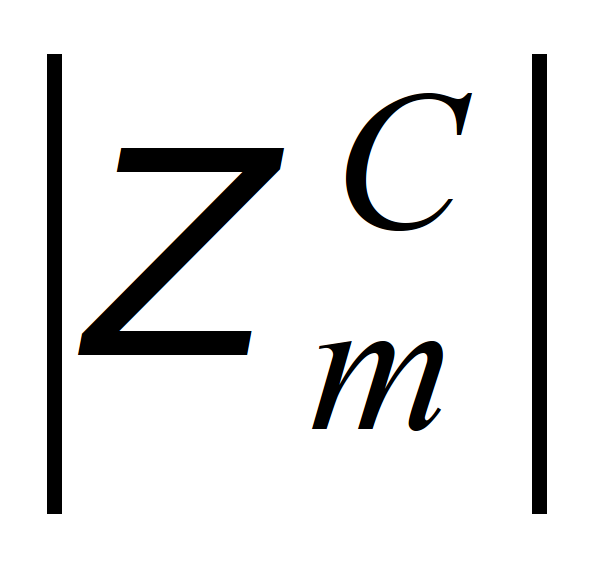
\includegraphics[width=0.4374in,height=0.4063in]{crypt-img/crypt-img47.png} 
означає число символів алфавіту криптограми, а \textit{n} --- її довжина. 

\textbf{\textit{Зауваження}}\textbf{.} Яку довжину криптограми в теоремах 4.2 і
4.3 можна вважати достатньою при практичному застосуванні? Це визначається
точністю співвідношення  \textit{H}(\textbf{M})  $?$\textit{  }\textit{nH}
$_{\infty }$. Як ми бачили в лекції 2, при \textit{n} біль-шому за 30 ця
приблизна рівність стає практично точною. Для \textit{n}\textit{ }меншого 10 у
наведеному вигляді формула для відстані однозначності дає значну помилку у бік
зменшення відстані однозначності. Щоб скоректувати у такому разі відповідь
треба враховувати відповідне зменшення надлишковості \textit{R} при невеликих
довжинах криптограм.

\textit{Наслідок формули Шеннона}. Якщо алфавіт шифрованого тексту співпадає з
алфавітом відкритого тексту (
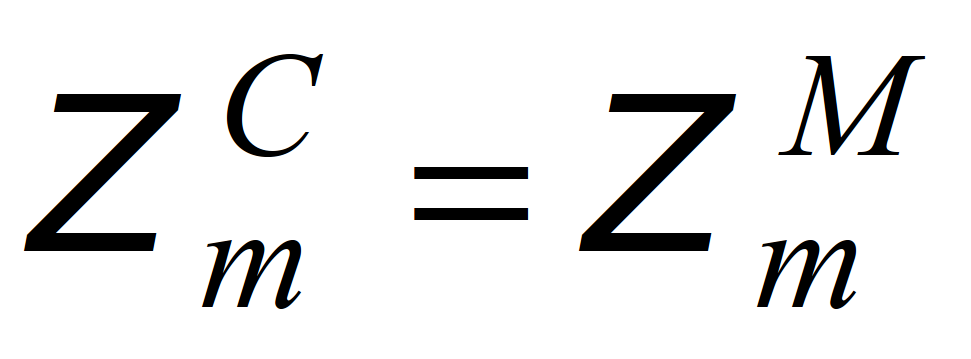
\includegraphics[width=0.9016in,height=0.3339in]{crypt-img/crypt-img48.png} ),
то надлишковість криптограми співпадає з надлишковістю відкритого тексту
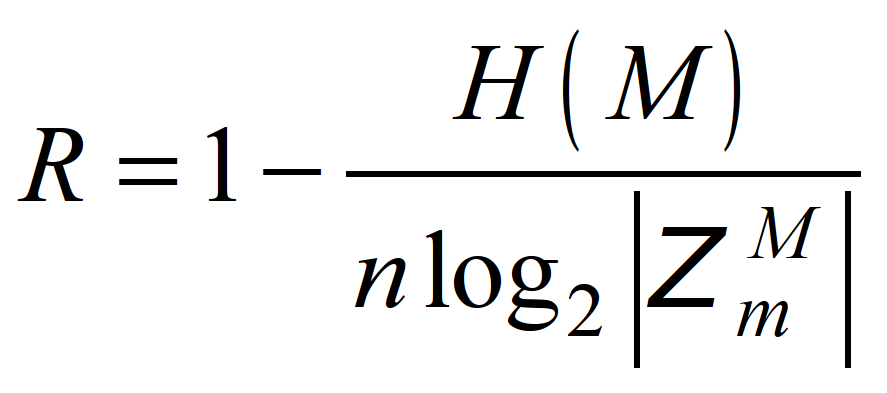
\includegraphics[width=1.6252in,height=0.7075in]{crypt-img/crypt-img49.png} . 
Як зазначалося у лекції 2, для iндоєвропейських мов надлишковість мови 
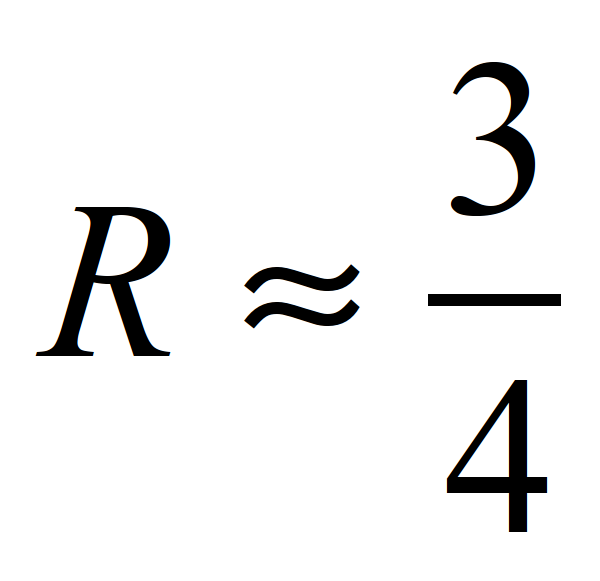
\includegraphics[width=0.5516in,height=0.5209in]{crypt-img/crypt-img50.png}   
(60-80\% залежно від тексту ).

Надлишковість в бітах на знак алфавіту 
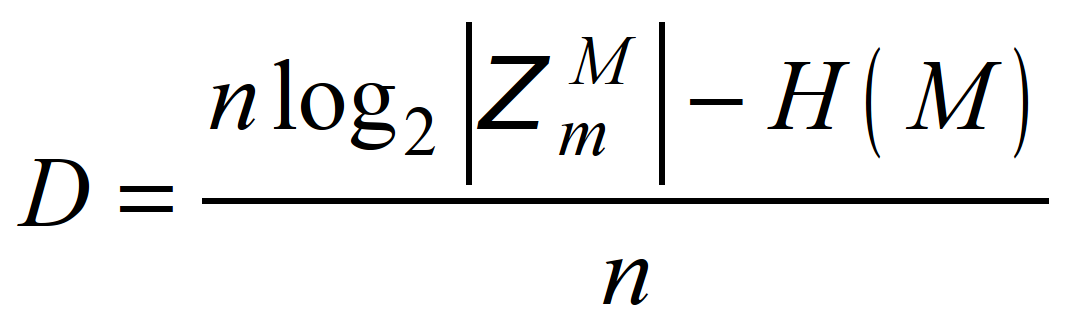
\includegraphics[width=2.122in,height=0.65in]{crypt-img/crypt-img51.png} . Якщо
  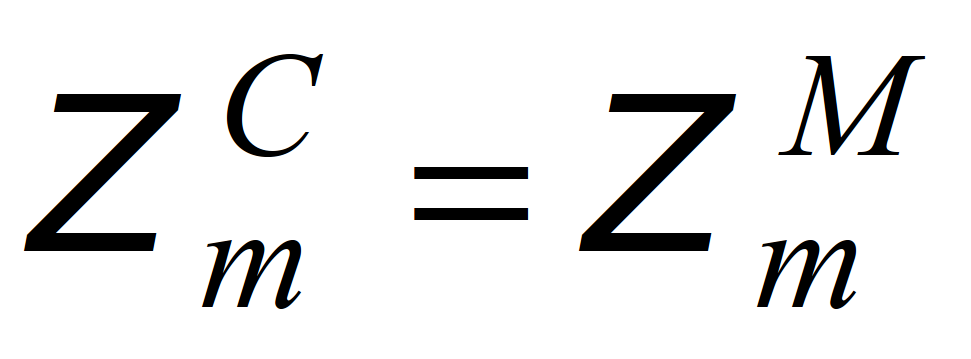
\includegraphics[width=0.9047in,height=0.3311in]{crypt-img/crypt-img52.png} ,
 то   $u\approx \frac{H(K)}D$.  Коли до того ж алфавіт ключа співпадає з
алфавітом шифрованого і відкритого текстів, а розподіл ключів  рівноймовірний,
то  
\includegraphics[width=0.5862in,height=0.5665in]{crypt-img/crypt-img53.png} , 
де  
\includegraphics[width=0.2291in,height=0.3335in]{crypt-img/crypt-img54.png}  ---
довжина ключа в символах алфавіту.

\textbf{\textit{Зауваження}}\textbf{.} Якщо при криптоаналізі використовуються
не всі статистичні та функціональні залежності мови, то надлишковість
\textit{R}\textit{ }у формулі для відстані однозначності треба брати меншою.
Так, якщо при криптоаналізі використовується тільки частота букв, то
надлишковість має бути як у моделі відкритого тексту М1 (дивись лекцію 2),
тобто \textit{R}=0.13 --- 0.15  і відстань однозначності  збільшиться в декілька
разів.  Очевидно, коли  \textit{R} $\rightarrow $ 0,\textit{  u}
$\rightarrow \infty $\textit{.  }Нагадаємо, що відстань однозначності --- це
усереднена за ключами і криптограмами достатньої  довжини характеристика. 
истовується тільки частота букв, то надлишковіссть має бути як

Поняття відстані однозначності дає орієнтир: чи можливо досягти успіху в повному
зламі криптосистеми за криптограмою певної довжини, чи ні.


\bigskip


\bigskip

\section{Контрольні питання}


\bigskip


\bigskip

\liststyleWWviiiNumx
\begin{enumerate}
\item Чи може бути зламана цілком таємна криптосистема по зашифрованому тексту
певної довжини?
\item Наведіть означення ненадійності ключа та ненадійності відкритого тексту.
Який зміст вкладається в ці поняття з точки зору теорії інформації?
\item Що таке функція ненадійності ключа?
\item Якою повинна бути ненадійність ключа, щоб його можна було знайти по
криптограмі, якщо виконати певний обсяг обчислень?
\item Що таке відстань однозначності?
\item Як впливає надлишковість на відстань однозначності?
\item В якому розумінні відстань однозначності є усередненою характеристикою?
\item Яка відстань однозначності у цілком таємної криптосистеми? 
\end{enumerate}

\bigskip


\bigskip


\bigskip

{\bfseries
ЛЕКЦІЯ  5}


\bigskip

{\centering\bfseries
МОНОАЛФАВІТНІ  ПІДСТАНОВКИ
\par}


\bigskip


\bigskip

\section{Підстановки на алфавіті. Підстановка як криптографічне перетворення}


\bigskip


\bigskip

Нехай \textit{Z}\textit{\textsubscript{m}} =
\{\textit{z}\textsubscript{1},\textit{z}\textsubscript{2},…\textit{z}\textit{\textsubscript{m}}\}
--- алфавіт відкритого та шифрованого текстів.

\textit{Означення.}\textit{ Підстановкою на алфавіті}\textbf{\textit{
}}\textbf{\textit{Z}}\textbf{\textit{\textsubscript{m}}} називається
взаємно-однозначне відображення  $\pi :Z_m\rightarrow Z_m$.

Інакше кажучи, будь-яка перестановка елементів
\textit{Z}\textit{\textsubscript{m}}\textsubscript{ } визначає підстановку на
\textit{Z}\textit{\textsubscript{m}}\textsubscript{ }. На множині підстановок
на \textit{Z}\textit{\textsubscript{m}} можна визначити операцію множення 
$\pi _1\cdot \pi _2$ (композиція підстановок).

З курсу дискретної математики вам відомо, що множина підстановок на
\textit{Z}\textit{\textsubscript{m}}\textsubscript{ } утворює групу відносно
операції множення. Одиницею цієї групи є тотожна підстановка; для кожної
підстановки \textit{\textgreek{p}}\textbf{ } існує обернена підстановка
\textit{\textgreek{p}}\textit{ }\textsuperscript{}-1} :
\textit{\textgreek{p}\textsf{\textit{ }}\textit{\textgreek{p}}
\textsuperscript{}-1}\textbf{ = }1. Ця група називається симетричною і
позначається SYM\textbf{(}\textit{Z}\textit{\textsubscript{m}\textbf{)}.
Кількість всіх підстановок на
\textit{Z}\textit{\textsubscript{m}}\textsubscript{ } дорівнює
\textit{m}\textit{!}.

Якщо задана підстановка \textbf{\textit{\textgreek{p}}}\textbf{\textit{ }} на
\textit{Z}\textit{\textsubscript{m}}\textsubscript{ }, то можна згідно з нею
букві ВТ  співставити букву ШТ. Але криптографічне перетворення повинно
задавати правило шифрування тексту будь-якої довжини \textit{n}.

Позначимо  $Z_m^n$ множину \textit{n}{}-грам над алфавітом
\textit{Z}\textit{\textsubscript{m}}.

\textit{Означення 5.1.}\textit{ Криптографічним перетворенням Т }називається
сімейство перетворень  $T=\;\{T^{(n)},\;n=1,2,\dots\}$,
де  $T^{(n)}:\;Z_{m}^{n}\rightarrow \;Z_m^n$\textsf{.}

\textit{Означення 5.2.}\textit{ Підстановка}\textbf{\textit{ }}(як
криптосистема) --- це криптографічне перетворення \textit{Т}\textbf{\textit{ }},
де  ${T^{(n)}=\{\pi _{1},\pi _{2},\dots,\pi
_{n}\}}$.

Тобто при шифруванні шифром підстановки тексту довжини \textit{n} перша буква ШТ
одержується з першої букви ВТ за допомогою підстановки на алфавіті
\textit{\textgreek{p}}\textsubscript{1}, друга --- за допомогою
\textit{\textgreek{p}}\textsubscript{2 }, ..., остання --- за допомогою
\textit{\textgreek{p}}\textit{\textsubscript{n}}.

Таким чином, криптографічне перетворення \textit{Т} задається ключем  ${k=\{\pi
_{1},\pi _{2},\dots\}}${}- нескінченною послідовністю
підстановок. Звернемо увагу на те, що букви при підстановці шифруються
незалежно одна від одної і кожна, взагалі кажучи, своєю підстановкою.

\textit{Означення 5.3.}\textit{ }Підстановка називається
\textit{моноалфавітною}, якщо\textbf{
}\textit{\textgreek{p}}\textit{\textsubscript{і}} =\textsf{\textit{
}}\textit{\textgreek{p}}\textbf{ , }\textit{і=1,2,...} (тобто всі букви
шифруються тією ж самою підстановкою). Якщо ж у послідовності   ${\{\pi
_{1},\pi _{2},\dots\}}$ не всі підстановки однакові, то
таке криптографічне перетворення називається \textit{поліалфавітною}
підстановкою.

Моноалфавітну підстановку ще називають \textit{шифром простої заміни}.

Підкреслимо, що при моноалфавітній підстановці одна й та сама буква алфавіту, що
зустрічається у ВТ, шифрується тією ж самою буквою ШТ незалежно від її місця у
тексті. Наприклад, якщо підстановка \textbf{\textit{\textgreek{p}}} переводить
букву „а” в  букву „м”, то де б не зустрілась буква „а” у ВТ, вона буде
зашифрована як „м”. У разі ж поліалфавітної підстановки одна й та сама буква
алфавіту може шифруватись по-різному в залежності від її місця у ВТ.


\bigskip


\bigskip

\section{Шифр Цезаря}


\bigskip


\bigskip

Найпростіша моноалфавітна підстановка --- це шифр Цезаря. Ототожнимо букви
алфавіту \textit{Z}\textit{\textsubscript{m}} з числами від\textbf{ }0 до
\textit{m-}1 і позначимо через \textit{x} довільну букву ВТ, а через \textit{y}
--- відповідну букву ШТ. Тоді в шифрі Цезаря   $y=x+b\;(\textmod\;m)$, де 
$0\le b\le m-1$ --- ключ (сам Цезар використовував ключ \textit{b}\textit{=}3).
В цьому випадку підстановка на алфавіті  $\pi $ є циклічним зсувом алфавіту
на  $b$ позицій вправо.

Для того, щоб знайти ключ, маючи лише ШТ, знайдемо
\textit{y}\textbf{\textit{\textsuperscript{*}}} - букву, що найчастіше
зустрічається у ШТ. Нехай \textit{x}\textbf{\textit{\textsuperscript{*}}} ---
буква алфавіту, що має найбільшу частоту у мові, якою написаний ВТ. Тоді, якщо
текст достатньо довгий, щоб у ньому проявилися закономірності мови,
найвірогідніше, що \textit{x}\textbf{\textit{\textsuperscript{*}}} зашифровано
у  \textit{y}\textbf{\textit{\textsuperscript{*}}}. Отже, маємо 
$y^{?}=x^{?}+b\;(\textmod\;m)$, звідки ключ 
$b=y^{?}-x^{?}(\textmod\;m)$.

Звичайно, існує деяка імовірність помилки при виборі образу
\textit{x}\textbf{\textit{\textsuperscript{*}}}, а отже, і при визначенні ключа
 $b$. Тоді потрібно взяти другу за частотою букву ШТ
\textit{y}\textbf{\textit{\textsuperscript{** }}}і спробувати ключ  
$b=y^{\text{**}}-x^{?}(\textmod\;m)$ і т.д., доки не одержимо
змістовний текст.


\bigskip


\bigskip


\bigskip


\bigskip


\bigskip


\bigskip

\section{Шифр афінної підстановки}


\bigskip


\bigskip

У шифрі Цезаря ключ може приймати всього \textit{m}\textbf{\textit{ }}значень,
де \textit{m }---\textit{ }потужність алфавіту. Оскільки  \textit{m} невелике, то
всі ключі можна досить швидко перебрати, інакше кажучи, шифр Цезаря має малий
ключовий простір. Розглянемо трохи складніший шифр --- шифр афінної підстановки:

{\raggedleft
  $y=\normalsubformula{\textax}+b\;(\textmod\;m)$  (5.1)
\par}

Тут ключем є пара чисел  $(a\;,b),\ 0<a\le m-1\;,\ 0\le b\le m-1$ , причому 
$a$ повинно бути взаємно простим з \textit{m}.

З (5.1)\textbf{ }одержуємо

{\raggedleft
  $x={a}^{'}y+b^{'}(\textmod\;m)$  (5.2)
\par}

де  $a^{'}=a^{-1}\textmod\;m$ --- обернений до  $a$ елемент в кільці
лишків за модулем \textit{m},   $b^{'}=-a^{'}b$.

Рівність (5.2)\textbf{ }має той самий вигляд, що й (5.1)\textbf{, }отже
шифрування і розшифрування здійснюються за однаковим алгоритмом, тільки з
різними параметрами. Умова взаємної простоти  $a$ з \textit{m} потрібна для
того, щоб існував обернений елемент  $a^{-1}$ і рівняння (5.1) при
фіксованому \textit{y} мало єдиний розв’язок  \textit{x} , тобто можливо було
однозначно розшифрувати ШТ. У противному випадку рівняння (5.1) має не єдиний
розв’язок  \textit{x} або взагалі його не має.

Афінна підстановка теж легко піддається криптоаналізу, хоча кількість ключів в
цьому шифрі значно більша, ніж у шифрі Цезаря, а саме 
\textit{\textgreek{f}}\textit{ (m) · }\textit{m} , де
\textit{\textgreek{f}}\textit{ (m)} --- функція Ейлера (кількість чисел менших за
\textit{m} і взаємно простих з ним). Нехай   $y^{?}$ і  $y^{\text{**}}$
- перша і друга за частотою букви ШТ,  $x^{?}$ і  $x^{\text{**}}$ -
відповідно найчастіша і наступна за нею за частотою букви мови.

Природно припустити, що при шифруванні  $x^{?}$ перейшла в  $y^{?}$, а 
$x^{\text{**}}$ --- в  $y^{\text{**}}$.

Складемо систему рівнянь:


\bigskip

{\centering
\textsf{ }
${\begin{matrix}\left\{ y^{?}=\normalsubformula{\text{ax}}^{?}+b\;\;\text{mod}\;m? \right.\left\{ y^{\text{**}}=\normalsubformula{\text{ax}}^{\text{**}}+b\;\;\text{mod}\;m? \right.\mathit{no}\hfill\null
\end{matrix}\{?}$\textsf{  }(5.3)
\par}


\bigskip

Відмітимо, що в цій системі невідомими є  $a$ і   $b$, а 
\textit{x}\textbf{\textit{ }}і\textbf{\textit{ }}\textit{ }\textit{y} --- відомі.

З (3)\textbf{ }маємо:

{\centering
\textsf{ }
$y^{?}-y^{\text{**}}=a\;(x^{?}-x^{\text{**}})\;\textmod\;m$\textsf{
 }(5.4)
\par}


\bigskip

Якщо пари  ${x^{?}\leftrightarrow y^{?},\;\;x^{\text{**}}\leftrightarrow
y^{\text{**}}}$ підібрані  вірно, то рівняння (5.4) має розв’язок  $a$.
Знаючи  $a$, з (5.3) знаходимо  $b$. Якщо ж ці пари не відповідають
дійсності, то (5.4) або не має розв’язку, або при всіх розв’язках (5.3),
розшифровуючи, одержимо беззмістовний текст. Тоді можна розглянути пари 
${x^{?}\leftrightarrow y^{\text{**}},\;\;x^{\text{**}}\leftrightarrow
y^{?}}$ або деякі інші пари серед невеликої кількості найчастіших букв ШТ і
ВТ.


\bigskip


\bigskip

\section{Загальний шифр простої заміни}


\bigskip


\bigskip

Розглянемо тепер довільну моноалфавітну підстановку, що визначається
підстановкою  на алфавіті  \textit{\textgreek{p}}\textbf{\textit{ }}. В цьому
випадку кількість ключів для латинського алфавіту дорівнює

{\centering
\textit{m}!\textit{ = }26!\textit{ $\approx$}\textsf{ }4
\textgreek{;}10\textsuperscript{26}\textit{,}
\par}

для кирилиці (якщо вважати, що алфавіт складається з 32 букв)

{\centering
32! $\approx$ 2,6 \textgreek{;}10\textsuperscript{35}.
\par}

Отже, якщо ключ записати у вигляді послідовності букв, то в латинському алфавіті
ключ буде мати довжину  log \textsubscript{2 }(26!) $\approx$ 88 біт
$\approx$22 букви  (для запису однієї букви потрібно log \textsubscript{2 }26
$\approx$ 4 біти), а в кирилиці довжина ключа  log \textsubscript{2 }(32!)
$\approx$ 118 біт $\approx$ 24 букви. При цьому букви в ключі мають бути
незалежними і рівномірно розподіленими. Якщо ж в якості ключів брати,
наприклад, змістовні тексти, то кількість ключів різко скоротиться, що призведе
до критичного зниження стійкості криптосистеми. Загальний шифр простої заміни є
яскравим прикладом шифру, який незважаючи на досить великий ключовий простір,
піддається криптоаналізу, хоча й не так легко, як у попередніх прикладах.

Знаходження однієї вірної пари   $x\leftrightarrow y$ мало що дає для
розшифрування тексту. Потрібно знаходити відповідності серед кількох найбільш
частих букв ВТ і ШТ, а також найменш частих букв. Крім того, існує багато
прийомів криптоаналізу, що межують з мистецтвом. Можна, наприклад, визначити
біграми, які часто зустрічаються у мові, а  біграми зворотного порядку --- рідко
(в англійській мові це, наприклад, ТН --- НТ, НЕ --- ЕН), а також біграми, що мають
велику і приблизно однакову частоту в прямому і зворотному порядку (RE --- ER), і
шукати відповідні за частотою  біграми ШТ.

Якщо є підстави припустити, що деяке слово неодноразово зустрічається в тексті,
можна шукати відповідну послідовність букв у ШТ (це особливо ефективно, коли в
слові повторюються букви). Цей метод має назву методу вірогідного слова. Існує
також багато інших прийомів.

Таким чином, моноалфавітна підстановка піддається криптоаналізу, тому що вона
зберігає \textit{статистичні властивості} мови --- частоти букв, біграм, слів і
т.д.

\textit{Означення 5.4.}\textit{ }Метод криптоаналізу, що базується на порівнянні
частот букв, біграм, слів і інших елементів тексту у ШТ і в мові, якою
написаний ВТ, називається \textit{частотним аналізом}.

Чим ближчий розподіл букв у ВТ до рівномірного, тим складніше застосовувати
частотний аналіз. Тому, як правило, ВТ перед шифруванням піддають деякому
перетворенню, що згладжує нерівномірність частот. Так, наприклад, видаляють
пробіл, що є найчастішою «буквою» алфавіту. Розподіл біграм більш рівномірний,
ніж розподіл букв. Тому часто ВТ розбивають на біграми і в якості алфавіту
розглядають множину біграм. Прикладами таких шифрів є афінна підстановка
біграм, а також шифр Плейфера.


\bigskip

\section{Шифр Плейфера}


\bigskip


\bigskip

Букви алфавіту розміщують у квадратній таблиці. Якщо кількість букв у алфавіті
не є повним квадратом, то деякі букви об’єднуть або до алфавіту додають
символи. Таблицю заповнюють по рядках: спочатку пишуть ключове слово (воно може
мати довжину від 1 до \textit{k}\textsuperscript{2} , де
\textit{k}\textsuperscript{ 2} --- кількість букв у таблиці). Далі записують
букви алфавіту, що не входять у ключове слово, в алфавітному порядку.
Наприклад, якщо в латинському алфавіті об’єднати букви I та J і вибрати
ключовим словом „LIBERTY”, то квадрат Плейфера буде мати вигляд:


\bigskip

{\centering\bfseries
L  I  B  E  R
\par}

{\centering\bfseries
T  Y  A  C  D
\par}

{\centering\bfseries
F  G  H  K  M
\par}

{\centering\bfseries
N  O  P  Q  S
\par}

{\centering\bfseries
U  V  W  X  Z
\par}


\bigskip


\bigskip

Певно, що у ключовому слові букви не повинні повторюватися.

При шифруванні ВТ розбивається на біграми, що не перетинаються. Попередньо між
буквами, що повторюються, вставляють деяку букву, яка має малу частоту і ніколи
не зустрічається двічі підряд, наприклад \textbf{\textit{Q}}. Тобто замість
слова, скажімо, \textbf{BUTTER} треба записати \textbf{BUTQTER}, а замість слів
\textbf{SENT TO}  --- \textbf{SENTQ TO}. Отже, при розбитті на біграми не
зустрінеться біграма з двох однакових букв. Можна замість \textbf{\textit{Q
}}використати деякий спеціальний символ, ввівши його до алфавіту.

Кожна біграма ВТ шифрується таким чином:

\liststyleWWviiiNumxxx
\begin{itemize}
\item якщо букви біграми стоять в одному рядку, то відповідна біграма ШТ
складається з букв, що стоять в тому ж рядку справа від даних. При цьому
вважається, що перший стовпчик стоїть справа від останнього. Наприклад, біграма
YC зашифрується як AD, а біграма FM --- як GF;
\item якщо букви біграми стоять в одному стовпці, то вона шифрується біграмою,
що складається з букв, які стоять в тому ж стовпці під даними; при цьому
вважається, що перший рядок знаходиться під останнім;
\item якщо букви біграми стоять у різних рядках і стовпцях, то відповідна
шифрована біграма складається з букв, що стоять у протилежних кутах
прямокутника, заданого даними буквами. Наприклад, біграма TQ буде зашифрована
як СN.
\end{itemize}
Кількість ключів у шифрі Плейфера дорівнює \textit{к}\textsuperscript{2}!  , але
деякі з них є еквівалентними, тобто однаково шифрують однакові ВТ.

Шифр Плейфера також піддається частотному аналізу, хоча й дуже копіткому. При
криптоаналізі використовують як частоти біграм, так і деякі обмеження і
закономірності, що випливають з правил шифрування.


\bigskip


\bigskip

\section{Шифрування за Хіллом}


\bigskip


\bigskip

Можна узагальнити шифр афінної підстановки на \textit{n}{}-грами (шифрування за
Хіллом). \textit{п}{}-грами ВТ і ШТ розглядаються як \textit{n}{}-вимірні
вектори над кільцем лишків \textit{Z}\textit{\textsubscript{m}}, а шифрування
відбувається за правилом

{\centering
 $\bar{y}=A\barx+\overlineb$,
\par}

де  $A$ --- невироджена матриця   $n\times n$, а  $\overlineb$ -
довільний вектор довжини \textit{n} над
\textit{Z}\textit{\textsubscript{m}}\textsubscript{ }; всі операції над
елементами матриці та компонентами векторів виконуються за  $\textmod\;m$.

На цьому прикладі видно, що границя між потоковими та блоковими шифрами досить
умовна: шифр Хілла можна розглядати і як потоковий, де елементами алфавіту є
\textit{n}{}-грами, і як блоковий з довжиною блока \textit{n}. Але підкреслимо
при цьому, що істотною відмінністю блокового шифру від потокового є те, що в
блоковому шифрі всі блоки шифруються однаково і незалежно один від одного, в
потоковому ж, взагалі кажучи, кожна буква може шифруватися в залежності від її
місця в тексті і від інших букв тексту, а також від того, як саме вони
шифруються.


\bigskip


\bigskip


\bigskip

\section{Контрольні питання}


\bigskip

\liststyleWWviiiNumxiv
\begin{enumerate}
\item Що таке підстановка на алфавіті і підстановка як криптографічне
перетворення?
\item Чим відрізняється поліалфавітна підстановка від моноалфавітної?
\item Дайте визначення шифру Цезаря, шифру афінної підстановки, загального шифру
простої заміни.
\item Скільки різних ключів має афінна підстановка, якщо в алфавіті 32 букви?
\item Блоковим чи потоковим шифром є шифрування за Хіллом?
\item Що таке частотний аналіз?
\end{enumerate}

\bigskip


\bigskip


\bigskip

{\bfseries
ЛЕКЦІЯ  6}


\bigskip

{\centering\bfseries
ПОЛІАЛФАВІТНІ  ПІДСТАНОВКИ
\par}


\bigskip


\bigskip

\section{Моделі вибору ключа}


\bigskip


\bigskip

В загальному випадку поліалфавітна підстановка визначається ключем ---
нескінченною послідовністю підстановок на алфавіті  $Z_m$ \{ ${\pi
_{1},\pi _{2},\dots}$ (означення підстановки на алфавіті
див. у лекції 5). Розглянемо три моделі вибору підстановок в цій послідовності.
В усіх трьох вважається, що підстановки  ${\pi _{1},\pi
_{2},\dots}$ вибираються незалежно одна від одної.

\textit{Модель1.  } $\pi _i$ ,  $i=1,2,\dots$ ---
довільні підстановки на  $Z_m$.  $P(\pi _i=\pi )=\frac1{m!}$,
тобто всі підстановки рівноімовірні.

 \textit{Модель 2.  } Кожна з підстановок  ${\pi
_{i},\;\;\;\;i=1,2,\dots}$ є шифром Цезаря (циклічним
зсувом алфавіту) із своїм ключем \textit{k}\textit{.}   $P(\pi _i$ є
циклічним зсувом на \textit{k} позицій $)=\frac1m,\;0\le k\le m-1$, тобто
всі циклічні зсуви  рівноімовірні. $ $

 \textit{Модель 3.  } $\pi _i$,  $i=1,2,\dots$ ---
шифри Цезаря,  $P(\pi _i$ є циклічним зсувом на \textit{k} позицій) 
$=p(k),\;$ де  $p(k)$ --- імовірність букви з номером  $k$ у мові. Ця
модель відповідає випадку, коли ключова послідовність є змістовним текстом. 


\bigskip

\section{Аперіодичні поліалфавітні підстановки}


\bigskip

Друга модель вибору ключа описує схему одноразового використання («одноразовий
блокнот») --- цілком таємну систему. (Звичайно, перша модель --- теж цілком таємна
система.) У разі двійкового алфавіту обидві моделі зводяться до вже згадуваного
шифру Вернама (див. лекцію 3). Доведення цілковитої таємності для цих двох
моделей аналогічне наведеному у лекції 3. Довжина ключа в розглядуваному шифрі
дорівнює довжині тексту, і ключ не можна стиснути. Символи ШТ 
$y_i,i=1,2,\dots$ будуть при цьому незалежними і
рівномірно розподіленими: 
${P(y=t)=P(x+k=t)=\overset{m-1}{\underset{s=0}{\sum
}}{P(x+k=t/k=s)P(k=s)}=\frac{1}{m}\overset{m-1}{\underset{s=0}{\sum
}}{p(t-s)=\frac{1}{m}}}$.

Якщо ж вибирати в якості ключа змістовний текст, то ми одержимо модель, близьку
до моделі 3. У зв’язку з надлишковіст
